\documentclass[12pt,a4paper]{report}

\usepackage{color}
\usepackage{showlabels}
\renewcommand{\showlabelfont}{\small\slshape\color{magenta}}
%\usepackage{showkeys}


\usepackage[utf8]{vietnam}
\usepackage{amsmath}
\usepackage{amsfonts}
\usepackage{mathtools,amssymb}
\usepackage{graphicx}
\usepackage{type1cm}
\usepackage{amsmath,amsxtra,amssymb,latexsym, amscd,amsthm}
\usepackage{url}


\usepackage{picinpar}
\usepackage{floatflt}
\usepackage{commath}
\usepackage{makeidx}
\usepackage{enumerate}
\usepackage{longtable}%
\usepackage{multicol}%
\usepackage[left=3.5cm,right=2.5cm,top=2.5cm,bottom=2.5cm]{geometry}

%\usepackage{indentfirst}
%\setlength{\parindent}{6.5ex}

\usepackage[graphicx]{realboxes}

\usepackage{algorithmic}
\usepackage[chapter]{algorithm}
\makeatletter
\renewcommand{\ALG@name}{Thuật toán}

\usepackage[sort&compress]{natbib}
%\usepackage{natbib}
%\bibliographystyle{abbrvnat}
%\setcitestyle{[author,open={(},close={)}]}

\usepackage[backref=page]{hyperref}

\usepackage{etoolbox}
\makeatletter
\patchcmd{\BR@backref}{\newblock}{\newblock(trang~}{}{}
\patchcmd{\BR@backref}{\par}{)\par}{}{}
\makeatother

\usepackage{filecontents}


\newtheorem{dly}{Định lý}[chapter]

\newtheorem{bde}[dly]{Bổ đề}
\newtheorem{hqua}[dly]{Hệ quả}

\theoremstyle{definition}
\newtheorem{gth}{Giả thiết}



\theoremstyle{definition}
\newtheorem{dng}{Định nghĩa}
\newtheorem{nx}{Nhận xét}
\newtheorem{gch}[dly]{Chú ý}
\newtheorem*{cm}{Chứng minh}
\newtheorem{hq}{Hệ quả}
\theoremstyle{definition}
\newtheorem{vd}[dly]{Ví dụ}
\newtheorem{bt}[dly]{Bài toán}
\newtheorem{kl}{Kết luận}
\theoremstyle{definition}
\newtheorem{tch}[dly]{Tính chất}


\def\n{\noindent}
\def\N{\mathbb{N}}
\def\R{\mathbb{R}}
\def\Z{\mathbb{Z}}
\def\p{\varphi}
\def\cc{\mathcal }
\def\ov{\overline}
\def\a{\alpha}
\def\lb{\lambda}
\def\va{\varepsilon}
\def\g{\gamma}
\def\V{\Vert}
\def\tR{\widetilde{R}}
\def\Re{\mathrm{Re}}
\def\re{\mathrm{Re}}

\DeclareMathOperator{\intt}{int}
\newcommand{\m}[1]{
\begin{bmatrix}
	#1
\end{bmatrix}}
\def\cA{\mathcal{A}}
\def\cC{\mathcal{C}}
\def\cP{\mathcal{P}}
\def\tu{\tilde{u}}
\def\R{\mathbb{R}}
\def\C{\mathbb{C}}
\newcommand{\pma}[1]{
	\begin{matrix}
		#1
\end{matrix}}
\newcommand{\hoac}[1]{\left[\begin{aligned}#1\end{aligned}\right.}
\newcommand{\heva}[1]{\left\{\begin{aligned}#1\end{aligned}\right.}

\setlength{\parindent}{0pt}

\begin{document}
\setlength{\baselineskip}{22 truept}
{\setlength{\unitlength}{1cm}}
%\addcontentsline{toc}{chapter}{Lời cảm ơn}
\centerline {\textbf{LỜI CẢM ƠN}}

Trong quá trình thực hiện và hoàn thành luận văn, tôi đã nhận được sự tạo điều kiện và động viên của thầy cô, bạn bè. Nhân dịp này, lời đầu tiên chúng tôi xin bày tỏ lòng biết ơn sâu sắc tới: Ban chủ nhiệm Khoa Toán - Lý - Tin, Phòng QLKH \& QHQT, các thầy cô trong tổ Bộ môn Giải tích, các bạn sinh viên lớp K55 ĐHSP Toán, đặc biệt là \textbf{TS. Hà Phi}, người thầy đã định hướng nghiên cứu, hướng dẫn chúng tôi thực hiện đề tài này.

Những ý kiến đóng góp, giúp đỡ động viên của quý thầy cô, bạn bè đã tạo điều kiện thuận lợi để chúng tôi hoàn thành đề tài. Nhân dịp này chúng tôi xin được bày tỏ lòng biết ơn về những sự giúp đỡ quý báu nói trên.  


 \textbf{Tôi xin chân thành cảm ơn}!


\hspace*{8.5cm}{\it Sơn La, tháng 5 năm 2017}\\
\hspace*{10cm} {\it Sinh viên thực hiện}\\
                 
\hspace*{10cm} {\bf Hoàng Việt Anh}

 \newpage

\begin{titlepage}
	\centerline{\fontsize{14pt}{18pt}\bf TRƯỜNG ĐẠI HỌC SƯ PHẠM HÀ NỘI}
	\centerline{\Large\bf KHOA TOÁN - TIN}
	\centerline{--------------------------o0o--------------------------}
	\vspace*{4cm}
	\centerline{\fontsize{14pt}{18pt}\bf LUẬN VĂN THẠC SĨ }
	\vspace*{2cm}
	
	\begin{center}
		\centerline{\fontsize{14pt}{18pt}\bf Tên đề tài}
	\end{center}
	\centerline{\fontsize{14pt}{18pt}\bf PHÂN TÍCH TÍNH CHẤT ỔN ĐỊNH} 
	\centerline{\fontsize{14pt}{18pt}\bf CỦA CÁC HỆ ĐỘNG LỰC CÓ TRỄ}
	\centerline{\fontsize{14pt}{18pt} \bf SỬ DỤNG PHƯƠNG PHÁP HÀM LAMBERT VÀ ỨNG DỤNG}
	\vspace*{0,2cm}
	
	
	\vspace*{4cm}
	\begin{center}
		\begin{tabular}{l l}
			\hspace*{-0,5cm}{\fontsize{14pt}{18pt}\bf \textit{Chuyên ngành}}&{\fontsize{14pt}{18pt}\bf : Toán Ứng Dụng}\\
			\hspace*{-0,5cm}{\fontsize{14pt}{18pt}\bf \textit{Mã số}}&{\fontsize{14pt}{18pt}\bf : 8.46.01.12 }\\
			\hspace*{-0,5cm}{\fontsize{14pt}{18pt}\bf \textit{Học viên}}&{\fontsize{14pt}{18pt}\bf : Nguyễn Thị Vân Anh}\\
			\hspace*{-0,5cm}{\fontsize{14pt}{18pt}\bf \textit{Giảng viên hướng dẫn}}&{\fontsize{14pt}{18pt}\bf : TS. Hà Phi}\\
		\end{tabular}
	\end{center}
	\vfill
	\centerline{\fontsize{14pt}{18pt}\bf HÀ NỘI - 2021}
\end{titlepage}
\tableofcontents

%\section{Lập công thức không gian trạng thái}
Ta xét hệ thống điều khiển với thời gian liên tục sau
\begin{align}
    \dot{x}(t) &= Ax(t) + Bu(t), \; x(t_0) = x_0 \label{ct2.1.1} \\ 
    y(t) &= Cx(t) + Du(t).\nonumber 
\end{align}
trong đó A là ma trận cỡ \emph{n $\times$ n}, B cỡ \emph{n $\times$ m}, C là \emph{r $\times$ n} và D cỡ \emph{r $\times$ m}. Vector \emph{x} biểu diễn trạng thái, \emph{u} là vector điều khiển và \emph{y} là đầu ra. Ta minh họa bằng sơ đồ khối sau:
%hinh 2.1
\begin{figure}[htp]
\centering
  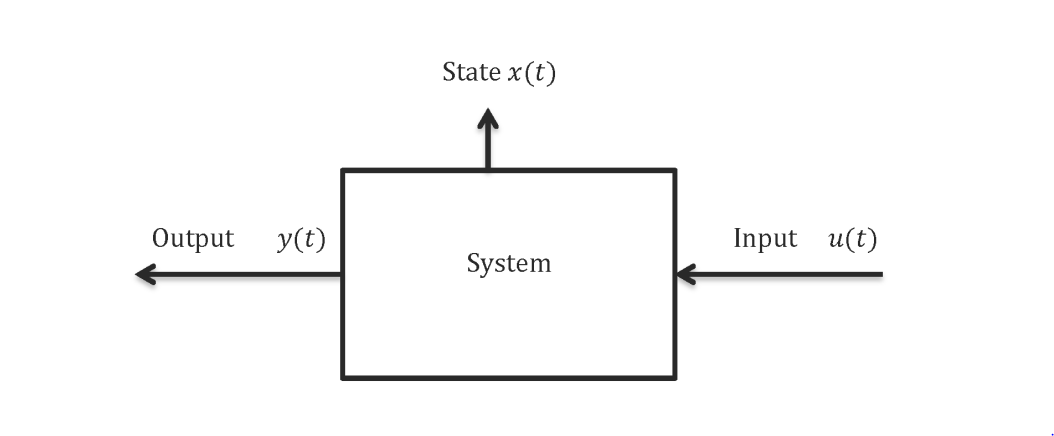
\includegraphics[width=13cm]{Anh1}
  \caption{Sơ đồ khối mô hình không-thời gian liên tục.}
  \label{fig:pic1}
\end{figure}
\begin{example}
Để minh họa rõ hơn việc lập công thức không gian trạng thái, ta xét hệ 2 vật nặng được nối với nhau bởi một lò xo và giảm chấn. Lực $\emph{u}$ tác động vào vật $M_1$, làm thay đổi vị trí $\emph{z}$ của vật $M_2$. Đầu vào của hệ này là lực tác động, đầu ra chính là vị trí của vật $M_2$. Ở đây thứ ta cần quan tâm chính là việc ta có thể điều khiển được vị trí của $M_2$.\\
Áp dụng định luật II Newton, ta có:
\begin{align}
    M_1\ddot{w} &= -b(\dot{w} - \dot{z}) - k(w - z) + u, \\
    M_2\ddot{z} &= b(\dot{w} - \dot{z}) + k(w - z).
\end{align}

\begin{figure}[htp]
\centering
  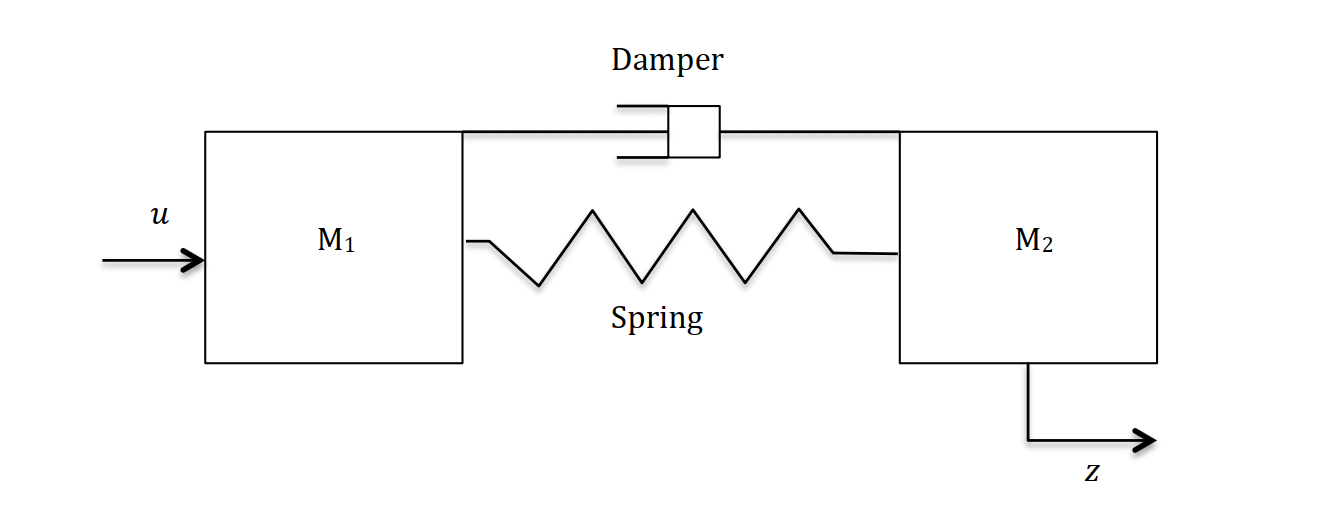
\includegraphics[width=13cm]{Anh2}
  \caption{Hệ vật lò xo giảm chấn.}
  \label{fig:pic2}
\end{figure}

Ở đây, b là hệ số tắt dần, w và z liên tục là sự dịch chuyển  $M_1$ và $M_2$, k là độ cứng của lò xo. Ta đưa hệ đạo hàm bậc 2 này về bậc 1 bằng cách:\\
Đặt $x_1$ = w, $\dot{x_1}$ = $\dot{w}$ = $x_2$, $x_3$ = z, $\dot{x_3}$ = $\dot{z}$ = $x_4$. Khi đó,
\begin{align}
\dot{x}_2 &= -\frac{b}{m_1}(x_2 - x_4) - \frac{k}{m_1}(x_1 - x_3) + u \label{ct2.1.4},  \\
\dot{x}_4 &= \frac{b}{m_2}(x_2 - x_4) + \frac{k}{m_1}(x_1 - x_3) + u, \\
y &= x_3.\label{ct2.1.6}
\end{align}
Ta viết lại \eqref{ct2.1.4}-\eqref{ct2.1.6} hệ dưới dạng ma trận
\begin{align}
    \begin{bmatrix}
        \dot{x}_1\\ \dot{x}_2\\ \dot{x}_3\\ \dot{x}_4
    \end{bmatrix}
     &= 
    \begin{bmatrix}
     0 & 1 & 0 & 0\\
     -\frac{k}{m_1} & -\frac{b}{m_1} & \frac{k}{m_1} & \frac{b}{m_1}\\
     0 & 0 & 0 & 1\\
     \frac{k}{m_2} & \frac{b}{m_2} & -\frac{k}{m_2} & -\frac{b}{m_2}
     \end{bmatrix}
     \cdot
     \begin{bmatrix}
     x_1 \\ x_2 \\ x_3 \\ x_4
     \end{bmatrix}
     + 
     \begin{bmatrix}
     0 \\ \frac{1}{m_1} \\ 0 \\ 0
     \end{bmatrix}
     \cdot u,\\
     y &= 
     \begin{bmatrix}
     0 & 0 & 1 & 0 
     \end{bmatrix}
     \cdot
     \begin{bmatrix}
     x_1 \\ x_2 \\ x_3 \\ x_4
     \end{bmatrix}.
\end{align}
Ta đưa hệ lò xo-giảm chấn này về dạng \eqref{ct2.1.1}
\bigskip
ta có
\newline
A = $\begin{bmatrix}
     0 & 1 & 0 & 0\\
     -\frac{k}{m_1} & -\frac{b}{m_1} & \frac{k}{m_1} & \frac{b}{m_1}\\
     0 & 0 & 0 & 1\\
     \frac{k}{m_2} & \frac{b}{m_2} & -\frac{k}{m_2} & -\frac{b}{m_2}
     \end{bmatrix}
\quad B = \begin{bmatrix}
     0 \\ \frac{1}{m_1} \\ 0 \\ 0
     \end{bmatrix}
\quad C = \begin{bmatrix}
     0 & 0 & 1 & 0 
     \end{bmatrix}
\quad D = 0.$
\end{example}

\section{Nghiệm không gian trạng thái}
Nếu ta đã biết vector \emph{u}, hệ \eqref{ct2.1.1} có thể giải được. Trước khi đi vào cụ thể, ta cần biết một vài định nghĩa \cite{5}.
\begin{definition}
Cho ma trận A cỡ n $\times$ n, khi đó ta định nghĩa \textbf{hàm mũ ma trận} là \[ e^{At} = \sum_{k = 0}^{\infty} \frac{(At)^k}{k!} .\]
\end{definition}
Hai điều lưu ý về hàm mũ ma trận:\\
1. \emph{$e^{A0} = A^0 = I$}. \\
2. \emph{$\frac{d}{dt}e^{At} = \sum_{k = 0}^{\infty} \frac{d}{dt} \frac{A^k t^k}{k!} = \sum_{k = 1}^{\infty} \frac{A^k t^{k-1}}{(k-1)!} = \sum_{k = 0}^{\infty}A\frac{A^k t^k}{k!} = Ae^{At}$}.\\
Ta biết nghiệm của bài toán giá trị ban đầu
\begin{align}
    \dot{x}(t) = Ax(t),\; x(t_0) = x_0, 
\end{align}
là x(t) = $e^{A(t-t_0)}x_0$.\\
Trở lại với phương trình tổng quát với u cho trước,
\begin{align}
    \dot{x}(t) &= Ax(t) + Bu(t), \; x(t_0) = x_0 \label{ct2.2.2} \\ 
    y(t) &= Cx(t) + Du(t). \label{ct2.2.3}
\end{align}
ta sẽ tìm nghiệm qua biến đổi Laplace.
\begin{definition}[Biến đổi Laplace]
Hàm f(x), x $\in$ [0,$\infty$) có biến đổi Laplace là tích phân $\mathcal{L}(f(x))(s)$ = $\hat{f}$(s) = $\displaystyle \int_1^\infty f(x)e^{-sx}dx$ với giá trị s $\in$ $\mathbb{C}$ mà tích phân có nghĩa.
\end{definition}
Hàm Laplace ngược của $\hat{f}$, ký hiệu bởi $\mathcal{L}^{-1} \hat{f}$ = f, là hàm f sao cho biến đổi Laplace của hàm đó chính bằng $\hat{f}$.\\
Để có thể tìm được nghiệm cho hệ phương trình \eqref{ct2.2.2} - \eqref{ct2.2.3}, ta biến đổi Laplace phương trình \eqref{ct2.2.2} và tìm nghiệm $\hat{x}$, cho ta kết quả là
\begin{align}
    \hat{x}(s) = (sI - A)^{-1} x_0 + (sI - A)^{-1} B \hat{u}(s). \label{ct2.2.4}
\end{align}
Áp dụng hàm Laplace ngược \eqref{ct2.2.4} cho ta nghiệm
\begin{align}
    x(t) &= L^{-1}((sI - A)^{-1} x_0) + L^{-1}((sI - A)^{-1} B \hat{u}(t)) \nonumber\\
         &= e^{A(t-t_0)}{x_0} + \displaystyle \int_{t_0}^t e^{A(t-s)}Bu(s)ds. \label{ct2.2.5}
\end{align}
Ta thay phương trình \eqref{ct2.2.5} vào phương trình \eqref{ct2.2.3} ta tìm được $y(t) = Ce^{A(t-t_0)}x_0 + \int_{t_0}^t Ce^{A(t-s)}Bu(s)ds + Du(t).$
\begin{definition}
Ma trận $e^{A(t-t_0)}$ được gọi là \textbf{ma trận chuyển trạng thái}.
\end{definition}
Nếu ta không biết hàm $\emph{u}$, ta có nhiều phương án điều khiển khác nhau để tìm ra hệ điều khiển có thể cho ra đầu ra mong muốn.

\section{Hàm truyền}
Hàm truyền sẽ cho ta thấy mối quan hệ giữa đầu vào và đầu ra của hệ thống và sự ảnh hưởng của nhiễu đối với đầu ra như thế nào.
Để tìm ra hàm chuyển của hệ \eqref{ct2.1.1}
\begin{align}
    \dot{x}(t) &= Ax(t) + Bu(t), \; x(0) = x_0 \label{ct2.3.1} \\ 
    y(t) &= Cx(t) + Du(t) \nonumber
\end{align}
ta sử dụng biến đổi Laplace như \eqref{ct2.2.4} để thu được nghiệm
\begin{align}
    \hat{x}(s) &= (sI - A)^{-1} x_0 + (sI - A)^{-1} B \hat{u}(s), \label{ct2.3.2}\\
    \hat{y}(s) &= C\hat{x}(s) + D\hat{u}(s). \label{ct2.3.3}
\end{align}
Trừ vế theo vế phương trình \eqref{ct2.3.2} cho phương trình \eqref{ct2.3.3} và đặt G(s) = $\frac{\hat{y}(s)}{\hat{u}(s)}$. Phương trình \eqref{ct2.3.3} trở thành 
\begin{align}
    \hat{y}(s) = G(s)\hat{u}(s), \nonumber
\end{align}
hay 
\begin{align}
    G(s) = \frac{\hat{y}(s)}{\hat{u}(s)}.
\end{align}
Hàm G(s) phản ánh tỷ số giữa đầu ra hệ thống $\hat{y}$(s) và đầu vào hệ thống $\hat{u}(s)$ và được gọi là hàm truyền ma trận hoặc đơn giản chỉ là ma trận truyền. Thành phần $G_{ij}$ trong ma trận biểu diễn hàm truyền từ đầu vào thứ j sang đầu ra thứ i. Hàm truyền này đại diện cho các thuộc tính của hệ thống và không đại diện cho độ lớn hoặc tính chất của các đầu vào. Nó cũng không phục vụ cho việc cung cấp bất kỳ thông tin nào về cấu trúc của hệ thống.\\
Một ưu điểm chính của việc sử dụng hàm truyền là chúng cho phép ta làm việc với một hệ thống phức tạp trong miền thời gian và biểu diễn nó như một hàm của một biến trong miền tần số. Thật không may, cách tiếp cận này chỉ hoạt động đối với các hệ thống đơn đầu ra - đơn đầu vào (SISO). Điều này có nghĩa là, đối với nhiều hệ thống đa đầu vào - đa đầu ra, thì sẽ có nhiều hàm truyền được sử dụng để biểu diễn mỗi quan hệ đầu vào - đầu ra. Cần lưu ý rằng, nhiều hệ thống có thể chia sẻ cùng một hàm truyền, không liên quan đến độ lớn của hệ thống hoặc tính chất của đầu vào.
\begin{definition}
Các điểm p mà tại đó hàm truyền G(p) = $\infty$ được gọi là các cực của hệ.
\end{definition}
Nếu G($\infty$) là một ma trận hằng thì hàm truyền được gọi là \textbf{chính} và nếu G($\infty$) = 0, hàm truyền được gọi là \textbf{chính ngặt}.
Chúng ta hãy sử dụng hệ thống giảm chấn khối lượng lò xo từ Ví dụ \eqref{ct2.1.1} để minh họa cách tìm hàm truyền của một hệ đã cho được mô tả bằng biểu diễn không gian trạng thái.
\begin{example}
Từ Ví dụ \eqref{ct2.1.1} ta có
\begin{math}
A = \begin{bmatrix}
     0 & 1 & 0 & 0\\
     -\frac{k}{m_1} & -\frac{b}{m_1} & \frac{k}{m_1} & \frac{b}{m_1}\\
     0 & 0 & 0 & 1\\
     \frac{k}{m_2} & \frac{b}{m_2} & -\frac{k}{m_2} & -\frac{b}{m_2}
     \end{bmatrix},
\quad B = \begin{bmatrix}
     0 \\ \frac{1}{m_1} \\ 0 \\ 0
     \end{bmatrix},\\
     C = \begin{bmatrix}
     0 & 0 & 1 & 0 
     \end{bmatrix},
\quad D = 0.
\\
\\
\\
Suy \; ra \\
G(s) = C(sI - A)^{-1}B + D = \begin{bmatrix}
0 & 0 & 1 & 0
\end{bmatrix}
\begin{pmatrix}
\begin{bmatrix}
s & 0 & 0 & 0 \\
0 & s & 0 & 0 \\
0 & 0 & s & 0 \\
0 & 0 & 0 & s.
\end{bmatrix}
- 
\begin{bmatrix}
0 & 1 & 0 & 0\\
-4 & -2 & 4 & 2\\
0 & 0 & 0 & 1\\
4 & 2 & -4 & -2
\end{bmatrix}
\end{pmatrix}^{-1}
\begin{bmatrix}
0\\
1\\
0\\
0
\end{bmatrix}.
\end{math}
\end{example}
Giản ước đi ta tìm ra 
\begin{align}
    G(s) = \frac{s + 2}{s^4 + 3s^3 + 6s^2}.\nonumber
\end{align}
\begin{definition}
Trong không gian thời gian - trạng thái biểu diễn ở \eqref{ct2.3.1}, ma trận
\begin{align}
    G(iw) = C(iwI - A)^{-1}B + D
\end{align}
được gọi là \textbf{ma trận phản hồi tần số}, $\omega \in \mathbb{R}$ chính \textbf{tần số}.
\end{definition}

\section{Tính điều khiển được và tính quan sát được}
Tính điều khiển và tính quan sát được là những khái niệm cơ bản của lý thuyết điều khiển. Để trình bày những khái niệm này, ta tham khảo trong mục \cite{5}
\begin{definition}
Hệ \eqref{ct2.1.1} 
\begin{align*}
    \dot{x}(t) &= Ax(t) + Bu(t),\\
    y(t) &= Cx(t) + Du(t)
\end{align*}
được gọi là có thể điều khiển được nếu hệ thống đạt được bất kì trạng thái bất kì $x_1 = x(t_1)$, trong thời gian hữu hạn $t_1$, từ bất kỳ trạng thái ban đầu x(0) bằng cách chọn điều khiển u(t), $0 \leq t \leq t_1$ phù hợp.
\end{definition}
Tính điều khiển của hệ thống \eqref{ct2.1.1}, được gọi là tính điều khiển của cặp (A, B). Định lý sau cung cấp các điều kiện có thể kiểm chứng được về việc một hệ thống có thể điều khiển được hay không.
\begin{theorem}\label{dly2.4.1}
Cho A  $\in \mathbb{R}^{n\times n}$  và  B  $\in \mathbb{R}^{n\times m}(m \leq n).$ Các điều sau đây là tương đương:
 \renewcommand{\theenumiii}{\roman{enumii}}
 \begin{enumerate}
    \item Hệ \eqref{ct2.1.1} có thể điều khiển được.
    \item Ma trận điều khiển $n \times nm$ là $C_M$ = $[B, AB, A^2B,...,A^{n-1}B]$ có đủ hạng dòng.
    \item Ma trận
    \begin{align*}
        W_C = \int_{0}^{t_1}e^{At}BB^{T}e^{A^{T}t}dt
    \end{align*}
không suy biến với bất kỳ $t_1$ > 0.
    \item Nếu ($\lambda$, x) là một cặp giá trị riêng và vector riêng tương ứng của $A^{T}$, thì $x^{T}B \ne$ 0.
    \item Rank(A - $\lambda$ I, B) = n với mọi giá trị riêng $\lambda$ của A.
    \item Các giá trị riêng của A - BK có thể được phân bố tùy ý bằng một lựa chọn thích hợp của K.
 \end{enumerate}
\end{theorem}
\newpage
\begin{definition}
Hệ thời gian liên tục \eqref{ct2.1.1} gọi là $\textbf{quan sát được}$ nếu tồn tại $t_1$> 0 sao cho trạng thái ban đầu x($t_0$) xác định duy nhất nếu biết u(t) và y(t) với mọi $0 \leq t \leq  t_1 $. 
\end{definition}
Tính quan sát được của hệ thống \eqref{ct2.1.1} được gọi là tính quan sát được của cặp (A, C).Tính đối ngẫu có nghĩa là cặp (A, C) có thể quan sát được nếu cặp ($A^{T}, C^{T}$) có thể điều khiển được. Do tính hai mặt của khả năng quan sát và khả năng điều khiển, khả năng quan sát có các đặc điểm tương tự như tính điều khiển được trong Định lý 2.4.1.
\begin{theorem}
Những điều sau đây là tương đương:
\renewcommand{\theenumiii}{\roman{enumii}}
\begin{enumerate}
    \item Hệ \eqref{ct2.1.1} có thể quan sát được.
    \item Ma trận của khả năng quan sát $O_M$ = $[C CA ... CA^{n-1} ]^{T}$ có hạng đủ.
    \item Ma trận
    \begin{align*}
        W_O = \int_{0}^{t_0}e^{A^{T}t}C^{T}Ce^{At}dt
    \end{align*}
không suy biến với mọi $t_1$ dương.
    \item Ma trận 
    \begin{math}
        \begin{bmatrix}
    \lambda I -A \\
    C
    \end{bmatrix}
    \end{math}
có hạng bằng n với mọi giá trị riêng của A.
    \item Nếu ($\lambda$, y) là 1 cặp giá trị riêng và vector riêng của A, thì $C_y \neq$ 0.
    \item Các giá trị riêng cho A - LC có thể được gán tùy ý bằng một lựa chọn thích hợp của L.
\end{enumerate}
\end{theorem}
Khả năng điều khiển và khả năng quan sát đóng vai trò quan trọng trong sự tồn tại của các nghiệm xác định dương và nửa xác định dương cho phương trình Lyapunov.
\begin{definition}
Ma trận A được gọi là \textbf{ma trận ổn định} nếu mọi giá trị riêng của A có phần thực âm thực sự.
\end{definition}
\begin{definition}
Cho A là một ma trận ổn định, thì 
\begin{align}
    C_G = \int_{0}^{t_1}e^{At}BB^{T}e^{A^{T}t}dt
\end{align}
gọi là \textbf{Grammian điều khiển.}
\end{definition}
\begin{definition}
Cho A là một ma trận ổn định, thì
\begin{align}
    O_G = \int_{0}^{\infty}e^{A^{T}t}C^{T}Ce^{At}dt 
\end{align}
được gọi là \textbf{Grammian quan sát.}
\end{definition}
\begin{theorem}\label{dly2.4.3}
Cho A là một ma trận ổn định. Grammian điều khiển $C_G$ thỏa mãn phương trình Lyapunov
\begin{align}
    AC_G + C_GA^{T} = -BB^{T}
\end{align}
và là đối xứng, xác định dương khi và chỉ khi (A, B) có thể điều khiển được.
\end{theorem}
\begin{theorem}\label{dly2.4.4}
Cho A là 1 ma trận ổn định. Grammian quan sát $O_G$ thỏa mãn phương trình Lyapunov
\begin{align}
    O_GA + A^{T}O_G = -C^{T}C
\end{align}
và là đối xứng, xác định dương khi và chỉ khi (A, B) có thể quan sát được.
\end{theorem}
Sau đây là một ví dụ minh họa tính toán của cả 2 giá trị $C_G$ và $O_G$.
\begin{example}
Trở lại hệ \eqref{ct2.1.1}, với 
\begin{align*}
    A = \begin{bmatrix}
        -4 & -8 & -12\\
        0 & -8 & -4\\
        0 & 0 & 0
    \end{bmatrix}, \; B = \begin{bmatrix}
        1\\
        1\\
        1
    \end{bmatrix}, \;  C = [1 \quad 1 \quad 1], \; D = 0.
\end{align*}
Ma trận A ổn định và sử dụng lệnh \textbf{lyap} trong  MATLAB để giải các phương trình Lyapunov trong Định lý 1.4.5 và 1.4.6, chúng ta tìm được
\begin{align*}
    C_G = \begin{bmatrix}
        0.1458 & 0.0208 & 0.0208\\
        0.0208 & 0.0833 & 0.0833\\
        0.0208 & 0.0833 & 0.0833
    \end{bmatrix} = O_G.
\end{align*}
Ta nhận thấy ma trận này có hai dòng bằng nhau nên định thức ma trận bằng 0, suy ra ma trận suy biến, nên (A, B) không điều khiển được và (C, D) không quan sát được.
\end{example}

\section{Tính ổn định hóa được và khả năng phát hiện được}
Một bộ điều khiển thường được thiết kế để ổn định hóa một hệ thống tuyến tính. Điều này được thực hiện bằng cách chọn một điều khiển $u$ thích hợp sao cho ma trận hệ đóng kín $(A - BK)$ ổn định, trong đó $K$ là ma trận phản hồi mà $u(t) = Kx(t)$. Trong phần này, chúng ta xác định tính ổn định hóa được của một hệ thống và trình bày các đặc điểm của hệ thống có thể được ổn định hóa được thông qua điều khiển phản hồi.\\
Đầu tiên chúng ta chọn hệ chưa điều khiển
\begin{align}\label{ct2.5.1}
    \dot{x}(t) = Ax(t), \quad x(0) = x_0.
\end{align}
\begin{definition}
Trạng thái cân bằng của hệ \eqref{ct2.5.1}, là vectơ $x_e$ thỏa mãn
\begin{align}
    Ax_e = 0.
\end{align}
Nếu ma trận A không suy biến, phương trình trên chỉ có nghiệm tầm thường $x_e$ = 0.
\end{definition}
\begin{definition}
Gọi $x_e$ là trạng thái cân bằng của \eqref{ct2.5.1}, thì $x_e$ được gọi là
\begin{enumerate}
    \item ổn định nếu với mỗi $\epsilon$ > 0 tồn tại $\delta$ > 0  sao cho $\norm{x(t) - x_e}$ < $\epsilon$,  $\forall$ t $\geq$ 0 nếu $\norm{x(t_0) - x_e} < \delta$.
    \item ổn định tiệm cận nếu trạng thái cân bằng ổn định và $\exists \delta > 0$ sao cho $\norm{x(t_0) - x_e} < 0$ dẫn đến $\displaystyle \lim_{x\to\infty} x(t) = x_e$.
\end{enumerate}
\end{definition}
Điều này có nghĩa là mọi nghiệm đúng của hệ nếu bắt đầu đủ gần điểm cân bằng ổn định tiệm cận, thì sẽ tiến gần đến điểm cân bằng khi thời gian tăng. Nên nếu $x_e = 0$ và \emph{A} không suy biến, hệ không ổn định được ở trên ổn định tiệm cận nếu $\emph{x(t)} \to 0 \; khi \; \emph{t} \to \infty.$
Các giá trị riêng của ma trận A trong \eqref{ct2.5.1} đặc trưng cho độ ổn định của hệ thống.
\begin{theorem}
Hệ thống \eqref{ct2.5.1} ổn định tiệm cận khi và chỉ khi mọi giá trị riêng của A có phần thực âm thực sự.
\end{theorem}
Cũng như với tính điều khiển, nghiệm của phương trình Lyapunov cũng đặc trưng cho tính ổn định của \eqref{ct2.5.1}.
\begin{theorem}
Hệ:
\begin{align*}
    \dot{x}(t) = Ax(t)
\end{align*}
ổn định tiệm cận khi và chỉ khi với ma trận M đối xứng dương bất kỳ, thì phương trình sau có nghiệm duy nhất
\begin{align*}
    XA + A^{T}X = -M.
\end{align*}
\end{theorem}
Xét hệ tuyến tính \eqref{ct2.1.1},
\begin{align*}
    \dot{x}(t) &= Ax(t) + Bu(t),\\
    y(t) &= Cx(t) + Du(t).
\end{align*}
Ta xét việc tìm nghiệm điều khiển \emph{u} để đưa hệ sang một trạng thái mong muốn. Điều đó có nghĩa là tìm 1 \textbf{ma trận phản hồi} $K$ sao cho $A - BK$ ổn định. Không phải mọi hệ có thể đưa về một trạng thái nhất định, nên điều quan trọng nhất của phần này là tìm ra điều kiện cần và đủ sao cho tồn tại một ma trận phản hồi ổn định.\\
Hơn nữa giả sử ta có thể tìm được mọi thông tin của trạng thái \emph{x(t)} ở mọi thời gian \emph{t} bất kỳ. Sử dụng điều khiển tuyến tính, ta suy ra 
\begin{align}
    u(t) = -Kx(t).
\end{align}
Trừ vế theo vế phương trình \emph{u(t) = -Kx(t)} cho phương trình \eqref{ct2.1.1} ta được \textbf{hệ kín}:
\begin{align}\label{ct2.5.4}
    \dot{x}(t) &= (A - BK)x(t),\\
    y(t) &= (C - DK)x(t).
\end{align}
Ta nhắc lại hệ không điều khiển được \eqref{ct2.5.1}
 ổn định khi ma trận A ổn định. Vậy nên việc ổn định hóa hệ \eqref{ct2.5.4} quy về việc tìm ma trận  $K$ sao cho $(A - BK)$ là ổn định. Nếu tồn tại một ma trận $K$, thì $K$ được gọi là \textbf{ma trận phản hồi} và ổn định hóa được, cặp ma trận (A, B) được gọi là \textbf{cặp ma trận ổn định hóa được}.\\
 Những định lý sau đây cho ta điều kiện cần và đủ để đánh giá việc có thể ổn định được ma trận cho 1 hệ đang xét.\\
 \begin{theorem}
  Những khẳng định sau là tương đương:
 \begin{enumerate}
     \item Cặp ma trận (A, B) là ổn định hóa được.
     \item Rank(A - $\lambda I$, B) = n, với mọi Re($\lambda$) $\geq$ 0.
     \item Với mọi $\lambda$ và x $\ne$ 0, nếu $x^{*}$A = $\lambda x^{*}$ và Re($\lambda$) $\geq$ 0 thì $x^{*}B \ne$ 0.
 \end{enumerate}
 \end{theorem}
 \begin{coroll}
 Nếu cặp (A, B) là điều khiển được,  thì nó cũng ổn định hóa được.
 \end{coroll}
 Lưu ý khả năng điều khiển suy ra khả năng ổn định chỉ là chiều suy ra mà không suy ngược lại.\\
 Cũng như khả năng quan sát được đối ngẫu với khả năng điều khiển được, khả năng ổn định được của hệ thống cũng đối ngẫu với khả năng phát hiện được.\\
 \begin{definition}
 Hệ được gọi là \textbf{phát hiện được} nếu tồn tại ma trận L sao cho với cặp ma trận (A, C) thì A - LC là ổn định.
 \end{definition}
\begin{theorem}
Các điều sau đây là tương đương:
\begin{enumerate}
    \item Cặp ma trận (A, C) là phát hiện được.
    \item Ma trận 
    $\begin{bmatrix}
        \lambda I - A \\
        C.
    \end{bmatrix}$
    có hạng đầy đủ, với mọi $Re(\lambda) \geq$ 0.
    \item Với mọi $\lambda$ và x $\ne$ 0 sao cho Ax = $\lambda$x và Re($\lambda) \geq$ 0, thì Cx $\ne$ 0.
    \item Cặp ma trận ($A^{T}$, $C^{T}$) là ổn định hóa được.
\end{enumerate}
\end{theorem}
Có thể thấy rằng một hệ thống có thể điều khiển được thì các giá trị riêng của hệ điều khiển đóng kín có thể được gán tùy ý (bài toán gán giá trị riêng). Vấn đề với việc chỉ định các giá trị riêng tùy ý đó là không có phương pháp luận để tìm một bộ điều khiển tối ưu sao cho các đặc điểm thiết kế hệ thống có thể đáp ứng một cách hiệu quả nhất có thể.\\
Điều này dẫn đến nhiều phương pháp điều khiển tối ưu ví dụ như điều khiển tối ưu tuyến tính bậc hai. Phương pháp này tối thiểu hóa hàm phạt bậc 2 đã được xác định trước. Tuy nhiên, lưu ý \cite{7} cho ta sự phát triển song song của điều khiển \hinf và điều khiển \emph{$H_2$} tối ưu hay còn được gọi là điều khiển dạng toàn phương tuyến tính Gauss.

\section{Chuẩn \hinf}
Trước tiên, hãy lưu ý rằng hàm truyền của một hệ thống ổn định bất kỳ được mô hình hóa bởi phương trình vi phân tuyến tính hệ số hằng là hàm hữu tỉ và có các cực nằm hoàn toàn trong nửa mặt phẳng bên trái và là giải tích trong nửa mặt phẳng bên phải. Một không gian của các hàm như vậy được gọi là không gian Hardy, ký hiệu là \hinf. Đối với hệ đa biến bất kỳ, hàm truyền G(i$\omega$) là một ma trận. Các giá trị kỳ dị của ma trận A, $\sigma_j$(A) được định nghĩa là
\begin{align*}
    \sigma_j(A) = \sqrt{\lambda_j(AA^{T})},
\end{align*}
trong đó $\lambda_j$(E) là giá trị riêng thứ j của ma trận E.
\newline
\newline
Chuẩn Euclid của ma trận là:
\begin{align*}
    \norm{A} = \displaystyle \max_{i}\sigma_i(A).
\end{align*}
Suy ra
\begin{align*}
    \norm{G(i\omega)} = \displaystyle \max_{i}\sigma_i(G(i\omega)) = \sigma_{max}(G(i\omega)).
\end{align*}
\begin{definition}
Chuẩn \hinf của hàm truyền G(s) được định nghĩa là
\begin{align}
    \norm{G}_{\infty} = \sup_{\omega \in \mathbb{R}}\sigma_{max}(G(i\omega)).
\end{align}
\end{definition}
\smallskip
Chuẩn này cung cấp một cách khác để phân tích tính ổn định của hệ thống, cụ thể là nếu G(s) $\in$ \hinf thì hệ thống ổn định. Như được mô tả trong \cite{15} cho trường hợp khi G là hữu tỉ, G $\in$ \hinf khi và chỉ khi G không có cực trong nửa mặt phẳng đóng bên phải.
\newpage
\chapter{Ước lượng hàm phân rã cho hệ thống tuyến tính có trễ}
\section{Đặt vấn đề}
Xét hệ thống tuyến tính đơn trễ với hệ số hằng (Linear Time Invariant Time-Delayed System) có dạng 
%
\begin{align}\label{1}
	& \dot{x}(t) = Ax(t) + A_dx(t-h) \mbox{ với mọi } t>0 , \\
	& x(0) = x_0 , \  x(t) = g(t) \ \mbox{với mọi } \ t \in [-h,0) , \notag
\end{align}
%
trong đó $A$ và $A_d$ là các ma trận hệ số cỡ $n \times n$, $x(t)$ là vectơ nghiệm cỡ $n \times 1$, $g(t)$ là hàm quỹ đạo ban đầu cỡ $n \times 1$, $t$ là biến thời gian và $h$ là độ trễ vô hướng cho trước. Một sự gián đoạn được cho phép tại $t = 0$ khi $g(0^-) \ne x(0) = x_0$. Mục tiêu là tìm giới hạn trên cho tốc độ phân rã $\a$ cũng như giới hạn trên cho hằng số $K$ sao cho ta có 
%
\begin{equation}\label{2}
	\Vert x(t)\Vert\leq Ke^{\a t} \Phi_h,
\end{equation}
%
trong đó $ \Phi_h=\sup\limits_{t_0-h\leq t\leq t_0}\{\Vert x(t)\Vert\}$ và $\Vert \cdot\Vert$ biểu thị chuẩn Euclid. Các điều kiện cho sự tồn tại của $K$ và $\a$ đã được thảo luận trong (\cite{Hal93}).
%
Một số lượng lớn các nghiên cứu đã được dành cho việc tìm hàm dạng $Ke^{\a t}\Phi$. Ví dụ hàm phân rã được dùng trong Hình \ref{fig:hinh-11}. Như trong hình vẽ, hàm phân rã $1$ cho ta ước lượng tốt hơn của $\a$ và $K$ so với hàm phân rã $2$.
%
Điều quan trọng là $K$ và $\a$ là một cặp và không thể ước lượng riêng lẻ chúng. Mặc dù tồn tại một số phương pháp tiếp cận miền tần số để tối ưu $\a$, một ước lượng tương ứng của $K$ không được trình bày trong cách tiếp cận đó. \\
%
Khi $h = 0$, $A_d = 0$ và phương trình vi phân có trễ (DDE) trong phương trình \eqref{1} rút gọn thành một phương trình vi phân thường (ODE), thì hàm phân rã của nó là
%
\begin{equation}\label{3}
	\Vert x(t)\Vert\leq e^{\mu (A) t}\Vert x(0)\Vert,
\end{equation}
%
trong đó $\mu (A) = \lim\limits_{\theta \to 0^+}\dfrac{\Vert I + \theta A\Vert -1}{\theta}$ là \emph{độ đo ma trận} (\cite{Hal93}).
%
Khi có thời gian trễ, vấn đề trở nên phức tạp hơn vì nghiệm $x(t)$ phụ thuộc không chỉ vào trạng thái ban đầu $x_0$ mà còn hàm quỹ đạo ban đầu  $g(t)$. Các cách tiếp cận cổ điển 
cho ta những ước lượng với một số hạn chế đáng kể. Ví dụ, cách tiếp cận theo chuẩn ma trận (\cite{Hal93}) cho ta ước lượng
%
\begin{equation}\label{4}
	K = 1 + \Vert A_d \Vert h  \ \mbox{ và } \ \a = \Vert A \Vert + \Vert A_d \Vert > 0 \ .
\end{equation}
%
Đối với các phương pháp đo lường ma trận (\cite{Leh94,Ni98}), $K$ được cố định bằng $1$, điều này làm cho ước lượng của $\a$ rất chặt chẽ. Ví dụ, xét quỹ đạo của hệ thống được biểu diễn trong Hình \ref{fig:hinh-11}. Nếu $K$ bằng $1$ thì hàm phân rã có giá trị bằng $1$ tại thời điểm $t=0$. Khi đó $\a$ phải dương để hàm phân rã bị giới hạn bởi đỉnh của quỹ đạo nghiệm chuẩn tại $t = 2$. Tuy nhiên, giá trị tối ưu của $\a$ rõ ràng là một số âm. \\

\begin{figure}[h!]
	\centering
	\includegraphics[scale= 0.7]{"./Hinh/Hinh11"}
	\caption[Ví dụ về hàm phân rã cho hệ có trễ bậc hai $\dot{x}(t) + Ax(t) + A_dx(t-h)= 0$, với $A = \m{0& 1\\ -1.25& -1}, A_d= \m{-0.1&0.6 \\ 0.2&0}, h = 1$ và $g(t)= \m{0\\1}$, với $t \le 0$]{Ví dụ về hàm phân rã cho hệ \eqref{1} với $A = \m{0& 1\\ -1.25& -1}, A_d= \m{-0.1&0.6 \\ 0.2&0}, h = 1$ và $g(t)= \m{0\\1}$, với $t \le 0$.}
	\label{fig:hinh-11}
\end{figure}

Ngoài ra, ta có thể áp dụng các phương pháp của Lyapunov để giải
quyết vấn đề về mặt tính toán. Sử dụng các phương pháp Lyapunov-Krasovskii cổ điển (xem \cite{Hal93}), các ước lượng của $K$ và $\a$ thu được là
%
\begin{equation}\label{5}
	K = \sqrt{\dfrac{c_2}{c_1}},  \ \a = - c_3,
\end{equation}
%
giả sử rằng tồn tại các hằng số dương $c_1, c_2, c_3$ sao cho\\
%
\begin{equation}\label{6}
	c_1 \Vert x(t) \Vert ^2 \le V(x_t) \le c_2 \Vert x_t \Vert ^2,
\end{equation}
%
và
%
\begin{equation}\label{7}
	\dot{V}(x_t) \le -2c_3 \Vert x(t) \Vert ^2,
\end{equation}
%
trong đó $x_t$ là hàm số được xác định bởi $x_t(\theta) := x(t+ \theta)$ với mọi $\theta \in [-h, 0]$ và $V(\cdot)$ là hàm Lyapunov-Krasovskii. Vì hạn chế vốn có của phương pháp Lyapunov, ước lượng tốc độ phân rã, $c_3$ sẽ không thể đạt được giá trị tối ưu. Ước lượng của $K$ cũng không đạt được giá trị tối ưu.\\
%
Chúng tôi có ý định khắc phục, hoặc giảm bớt những hạn chế vốn có trong các phương pháp đo lường ma trận và các phương pháp Lyapunov bằng cách áp dụng phương pháp hàm Lambert W. 
Mục tiêu là sử dụng biểu diễn dạng chuỗi cho công thức nghiệm của hệ \eqref{1} để đưa ra một ước lượng mới và tốt hơn cho hàm phân rã.

\section{Hàm Lambert W}
Hàm Lambert W là hàm số $W(z)$, $\mathbb{C} \to \mathbb{C}$, được định nghĩa là nghiệm của phương trình
\begin{equation}\label{eq2}
	W(z) \mathrm{e}^{W(z) }=z.
\end{equation}
Đây là một hàm đa trị, nghĩa là với mỗi $z \in \mathbb{C}$ thì có vô số nghiệm của \eqref{eq2}. Để nhận diện giá trị này, một nhánh số được gán, ta gọi $W_k(z)$ là nhánh thứ $k$ của hàm Lambert của $z$. Nhánh cắt được xác định bằng cách mỗi nhánh có một miền xác định riêng biệt \cite{Cor96}. Với $z \in \R$, chỉ có hai nhánh cho giá trị thực. Nhánh chính $W_0(z)$ có giá trị thực với $z \ge \dfrac{-1}{e}$ và miền giá trị của nhánh này là $[-1;\infty)$. Nhánh $W_{-1}(z)$ có giá trị thực với $\dfrac{-1}{e} \le z < 0$, và miền giá trị của nó là $(-\infty; -1]$. Hai nhánh này được biểu diễn ở Hình $1.2$.
Một nghiên cứu toàn diện về định nghĩa và tính chất của hàm Lambert W được tìm thấy trong \cite{Cor96}.
\begin{figure}[h!]
	\centering
	\includegraphics[scale= 0.7]{"./Hinh/Hinh 1"}
	\caption[Hai nhánh thực của hàm Lambert W]{Hai nhánh thực của hàm Lambert W}
	\label{fig:hinh-1}
\end{figure}
Bây giờ, ta sẽ định nghĩa ma trận của hàm Lambert W. \\
Xét một ma trận $H \in \C ^{n\times n}$, có phân tích Jordan là $H = ZJZ^{-1}$, với $J = \mathrm{diag} (J_1(\lb_1),J_2(\lb_2), \cdots , J_p(\lb_p) )$ và $Z$ là một ma trận khả nghịch. Ma trận hàm Lambert W cho mỗi khối Jordan $J_i$ cỡ $m$ được định nghĩa bởi
\begin{equation}\label{eq3}
	W_k(J_i) := \begin{bmatrix}
		W_k(\lb_i)  & W'_k(\lb_i) & \cdots & \dfrac{1}{(m-1)!} W_k ^{m-1}(\lb_i)\\
		0 & W_k(\lb_i) & \cdots & \dfrac{1}{(m-2)!} W_k ^{m-2}(\lb_i)\\
		\vdots  & \vdots  & \ddots & \vdots  \\
		0 & 0 & \cdots & W_k(\lb_i)
	\end{bmatrix} 
\end{equation}
và ma trận hàm Lambert của $H$ được định nghĩa bởi
\begin{equation}\label{eq4}
	W_k(H) := Z \ \mathrm{diag} (W_k(J_1(\lb_1),W_k(J_2(\lb_2), \cdots , W_k(J_p(\lb_p) )) \ Z^{-1}.
\end{equation}
Mọi ma trận được định nghĩa bởi \eqref{eq4}, với $k = 0, \pm 1, \pm 2, \cdots$ thỏa mãn
%
\begin{equation}\label{eq5}
	W_k(H) \mathrm{exp}	(W_k(H)) = H.
\end{equation}
%		
Định nghĩa chuẩn ở trên dẫn đến cùng một nhánh $k$ của hàm Lambert W được sử dụng trong tất cả các khối Jordan. Điều này là không cần thiết để có một nghiệm của \ref{eq5}. Từ $W_0(0)= 0$ và $W_k(0) = \infty$ với $k \ne 0$, ta điều chỉnh định nghĩa chuẩn để tránh sự vô hạn giá trị. Trường hợp đặc biệt này được gọi là trường hợp nhánh chuyển mạch, được định nghĩa trong \cite{Yi10} . Chi tiết hơn, $W_k(H)$ sử dụng giá trị $k$ cho những khối Jordan với $\lb \ne 0$ và $0$ cho những khối Jordan với $\lb = 0$. Định nghĩa này được sử dụng trong Chương \ref{Chap2}.
Bằng cách tương tự, giả sử rằng khi tính toán nhánh chính $e ^{-1}$ không là giá trị riêng của $H$ ứng với khối Jordan có số chiều lớn hơn $1$. Điều này được yêu cầu để vượt qua khó khăn bởi thực tế rằng $W'_0(e ^{-1})$ không xác định. Hạn chế này làm giảm vẻ đẹp của định nghĩa ma trận hàm Lambert W nhưng không ảnh hưởng đến hiệu quả của của việc sử dụng nó.



\section{Giải phương trình vi phân có trễ sử dụng hàm Lambert W}
\subsection{Trường hợp vô hướng}
Với trường hợp vô hướng, ta có phương trình
\begin{equation}\label{eq6}
	\dot{x}(t)=ax(t) + a_dx(t -h).
\end{equation}
Phương trình đặc trưng có dạng
\begin{equation}\label{eq7}
	s - a - a_d e ^{-s h} = 0.
\end{equation}
Nghiệm của \eqref{eq7} có thể được biểu diễn về hàm Lambert W theo các bước đơn giản (xem \cite{Yi10}) có dạng 
\begin{equation}\label{eq8}
	s_k = \dfrac{1}{h}W_k(a_d h e^{-ah})+a,
\end{equation}
trong đó $k = 0, \pm 1, \pm2, \cdots$ là chỉ số của các nhánh của hàm Lambert được sử dụng. Mỗi nghiệm trong số vô hạn các nghiệm của \eqref{eq7} tương ứng với một nhánh của hàm này.\\
Năm 2006, Shinozaki \& Mori đã chứng minh rằng trong số các nghiệm của \eqref{eq8}, nghiệm tương ứng với nhánh chính $k =0$ luôn có phần thực lớn nhất, do đó nó là nghiệm trội của phương trình. Do đó, để phương trình \eqref{eq6} ổn định, điều kiện cần và đủ  là $\Re(s_{0}) < 0$.

\subsection{Trường hợp bậc cao hơn}
Xét hệ phương trình \eqref{1} với $A, A_d \in \R^{n\times n}, h > 0$. Các bước sau đây được trình bày trong \cite{Yi10} nhằm tính toán các giá trị riêng bằng cách sử dụng ma trận hàm Lambert W. Phương pháp được đề xuất dựa trên việc tìm nghiệm của phương trình
\begin{equation}\label{eq10}
	S-A-A_d \exp (-Sh)=0,
\end{equation}
trong đó $S \in \C^{n\times n}$. Biến đổi \eqref{eq10} ta được
\begin{equation*}
	(S - A) \exp \left( (S - A) h + A h \right) = A_d.
\end{equation*}
Giả sử ta tìm được một ma trận $Q$ sao cho
\begin{equation*}
	\exp \left((S-A) + Ah \right) = \exp \left( (S-A) h \right)Q^{-1}.	
\end{equation*}
Khi đó ta có
\begin{equation}\label{eq11}
	h (S -A)\exp((S-A)h)= h A_d Q.
\end{equation}
Đặt $M : = h A_dQ$, ta thấy rằng với mỗi $k \in \Z$ thì
\begin{equation}\label{eq12}
	S_k = \dfrac{1}{h}W_k(M) + A 
\end{equation}
là một nghiệm của \eqref{eq11}. Bằng cách thay \eqref{eq12} vào \eqref{eq11}, ta thu được biểu thức sau
\begin{equation}\label{eq13}
	W_k(M)\exp (W_k(M)+Ah)-h A_d=0.
\end{equation}
%
Đến đây có hai cách tiếp cận khác nhau để tìm $S_k$, trong đó \eqref{eq13} được coi như là phương trình phi tuyến của biến số $M$ (\cite{Yi10}) hay biến số $W_k(M)$ (xem \cite{Wim15,GiU19}). Các bước tính nghiệm đặc trưng của hệ được cho bởi thuật toán sau. 

\begin{tht} \label{tht1}
	Lặp lại với $k = 0;\pm 1; \pm2; \cdots$\\
	(1) Giải phương trình phi tuyến
	\begin{equation}\label{eq14}
		W_k(M)\exp (W_k(M)+Ah)-h A_d=0,
	\end{equation}
	để tìm $M_k$, với $M_k = h A_d Q_k$.\\
	(2) Tính $S_k$ tương ứng với $M_k$ vừa tìm được
	\begin{equation}\label{eq15}
		S_k= \dfrac{1}{h }W_k(M_k)+A.
	\end{equation}
	(3) Tính các giá trị riêng của $S_k$.
\end{tht}

\noindent Để hệ \eqref{1} ổn định thì mọi giá trị riêng phải có phần thực âm. Việc tính nghiệm cho tất cả các nhánh là điều không thể. Để giải quyết khó khăn này, người ta giả sử rằng với bất kì nhánh $k$ nào của ma trận hàm Lambert, chỉ tồn tại duy nhất nghiệm $M_k$ của \eqref{eq14} tương ứng với ma trận $S_k$. Giả định này dựa trên quan sát từ nhiều ví dụ thực tế, dẫn đến một giả thuyết mạnh hơn sau đây \cite{Yi10,YiJune12}.

\begin{gth}\label{Hypo1}
Các giá trị riêng trội nhất nằm trên $m$ nhánh chính của hàm Lambert W trong đó $m$ là số khuyết của ma trận $A_d$. Cụ thể hơn, với mọi $i \in \mathbb{Z}$ ta có
\begin{equation}\label{hypothesis}
\max  \left\{ \Re(eig(S_i)), \ -m\leq i \leq m \right\} = \max \{ \Re(eig(S_i)), \ i\in\Z \} \ .  
\end{equation}
\end{gth}

\begin{hqua} Giả sử rằng Giả thiết \ref{Hypo1} được thỏa mãn cho hệ \eqref{1}. Khi đó, nếu $\mathrm{rank}(A_d) \geq 1$ 
thì giá trị riêng trội nhất của hệ \eqref{1} chính là giá trị riêng của ma trận $S_0$ tương ứng với nhánh chính của hàm Lambert trong Thuật toán \ref{tht1}.
\end{hqua}

\section{Ước lượng hàm phân rã của hệ có trễ}
Xét hệ phương trình \eqref{1}. Nghiệm của \eqref{1} có thể viết được dưới dạng sau (\cite{Yi10})
%
\begin{equation}\label{8}
	x(t) = \sum_{k = -\infty}^{\infty} e^{S_kt}C_k^I,
\end{equation}
%  
trong đó $S_k$ được tìm bằng cách sử dụng Thuật toán \ref{tht1}. Ở đây $S_k$ và $Q_k$ là ma trận cỡ $n \times n$, $C_I^k$ là véc tơ cỡ $n \times 1$ và được xác định bởi hàm quỹ đạo ban đầu $g(t)$ và $x_0$. Theo \cite[Phụ lục A]{Dua12} nghiệm tổng quát của hệ \eqref{1} có thể được viết dưới dạng
%
\begin{subequations}
\begin{equation}\label{11}
	x(t) = \underbrace{\sum_{k = -\infty}^{\infty} e^{S_k t} \left( \sum_{j=1}^{n} T^I_{kj} L^I_{kj} \right)x_0}_{:= P_1} - \underbrace{\sum_{k = -\infty}^{\infty} e^{S_k t} \sum_{j=1}^{n} \left(T^I_{kj} L^I_{kj} A_d G(\lb_{kj}) \right)}_{:=P_2},
\end{equation}
%
trong đó
%
\begin{align}\label{12}
	&\lb_{kj} :=eig(S_k), j = 1,2,\cdots, n,\\
%
	&G(\lb_{kj}):= \int \limits^h_0 e^{-\lb_{kj}h } g(s - h) ds, \\
%	
	&L^I_{kj} := \lim\limits_{s\to \lb_{kj}}	\left\{ \dfrac{\frac{\partial }{\partial s} \prod_{j=1}^{n} (s - \lb_{kj})}{\frac{\partial }{\partial s} \text{det} (s I + A + A_d e^{-sh})} adj(s I + A + A_d e^{-sh}) \right\},\\
% 
	& \tR^{I^+}_k := \begin{bmatrix}
		T_{k1}^I & T_{k2}^I & \cdots & T_{kn}^I
\end{bmatrix} = {R^I_k}^*(R^I_k {R^I_k}^*)^{-1}, \\
%
	& R_{kj}^I := adj (\lb_{kj}I - S_k), \tR_k^I = \m{R^I_{k1} \\R^I_{k2} \\  \cdots \\R^I_{kn} },
\end{align}
% 
\end{subequations}
trong đó $\tR_k^{I^+}$ là nghịch đảo mở rộng Moore-Penrose cỡ $n \times n^2$, ${R^I_k}^*$ là ma trận chyển vị liên hợp $n \times n^2$ của $\tR^I_k$ và $T_{kj}^I$ là khối vuông thứ $j$ của $\tR_k^{I^+}$.

\begin{dly}\label{dly1}
Giả sử rằng hệ \eqref{1} thỏa mãn Giả thiết \ref{Hypo1}. Bên cạnh đó ta cũng giả sử tồn tại các số thực $\a, K_1, K_2, K_3$ và $K_4$ sao cho
\begin{align}\label{17}
 \a = \max  \left\{ \Re(eig(S_i)), \ -m\leq i \leq m \right\} , 
\end{align}
\begin{subequations}\label{18}
\begin{align}
	&K_1 = \sup\limits_{0 \le t <h}   \underbrace{\left \Vert e^{(-A - \a I)t} \right\Vert}_{=:J_1(t)},\\
 \label{125b}
	&K_2 = \lim\limits_{N \to \infty} \sup\limits_{t \ge h} \underbrace{\left\Vert \sum_{k=-N}^{N} e^{(S_k-\a I)t} \sum_{j=1}^{n} T^I_{kj}L^I_{kj} \right\Vert }_{=:J_2(N,t)},    \\
	   &K_3 = \sup \limits_{0 \le t <h}  \underbrace{ \int_0^t \left\Vert e^{(-A-\a I)t +A h }A_d \right\Vert ds }_{=:J_3(t)} ,\\
 &K_4 = \lim\limits_{N \to \infty} \sup\limits_{t \ge h} \underbrace{ \int_{0}^{h} \left \Vert \sum_{k=-N}^{N} e^{(S_k-\a I)t} \sum_{j =1}^{n} \left(T^I_{kj}L^I_{kj}A_de^{\lb_{ki}s } \right) \right \Vert ds }_{=:J_4(N,t)},
\end{align}
\end{subequations}
%
trong đó $m$ là số khuyết của $A_d$ và $eig(S_i)$ là các giá trị riêng của $S_i$. 
Khi đó, nghiệm $x(t)$ của phương trình \ref{1} thỏa mãn ước lượng $\Vert x(t) \Vert \le Ke^{\a t}\Phi_h$ với mọi $t >0$ trong đó 
$\Phi_h := \sup\limits_{-h \le t \le 0} \left\{\Vert x(t) \Vert \right\} $ và $K := \max (K_1, K_2) + \max(K_3, K_4)$.
\end{dly}
\begin{cm} Rõ ràng Giả thiết \ref{Hypo1} cho ta tốc độ phân rã tối ưu của $\a$ chính là giá trị $\a$ trong \eqref{17}. 
%	
Ước lượng giá trị tối ưu của hệ số $K$ sao cho $\V x(t) \V \le K e^{\a t} \Phi_h$ trong đó $\Phi_h := \sup\limits_{-h \le t \le 0} \V x(t) \V$. 	
Lấy chuẩn cả hai vế của phương trình \eqref{11} ta được
\begin{align}\label{23}
	\V x(t) \V \le \V P_1(t) \V + \V P_2(t)\V \ .
\end{align}	
%
Lưu ý rằng với $t \in [0,h)$, ta có $x(t-h)=g(t-h)$ đã biết, vì vậy \eqref{1} trở thành
\begin{align}\label{24}
	\dot{x}(t) + Ax(t) = -A_dg(t-h) \mbox{ với mọi } t\in [0,h).
\end{align}
%
Mặt khác ta có các ước lượng sau với mọi $t \in [0,h)$
%
\begin{align}\label{25}
	\V P_1(t) \V &\le \V e^{(-A - \a I)t}x_0 \V e^{\a t} \le K_1 e^{\a t}\Phi_h, \\
	\V P_2(t) \V & \le \int_{0}^{t}\V -e^{-A(t-s )}A_d \V \cdot \V g(s  - h) \V ds  \notag\\
	&\le \int_{0}^{t}\V -e^{(-A - \a I)t + As }A_d \V \cdot \V g(s  - h) \V e^{\a t}ds  \notag\\
	&\le K_3e^{\a t}	\Phi_h.
\end{align}
%
Với $t\in [h,+\infty)$ ta có
\begin{align}\label{27}
	\V P_1(t) \V &= \lim\limits_{N \to \infty} \left \V \sum_{k=-N}^{N}  e^{(S_k-\a I)t} \sum_{j =1}^n T^I_{kj}L^I_{kj}x_0 \right \V e^{\a t} \notag\\
	& \le \lim \limits_{N \to \infty}  \sup \limits_{t \ge h} \left \V \sum_{k=-N}^{N}  e^{(S_k - \a I)t} \sum_{j =1}^n T^I_{kj} L^I_{kj} \right \V e^{\a t} \V x_0 \V.
\end{align}
Do đó $\V P_1(t) \V \le K_2 e^{\a t} \Phi_h$ với $t \in [h,\infty)$. Tương tự,
\begin{align}\label{28}
	\V P_2(t)\V &= \lim\limits_{N \to \infty} \left\V  \sum_{k=-N}^N e^{(S_k - \a I)t} \sum_{j =1}^n (T^I_{kj}L^I_{kj}A_d \int_0^h e^{\lb_{ki}s } g(s  - h) ds )   \right\V \notag \\
	& \le \lim\limits_{N\to \infty} \left\V \int_0^h  \sum_{k=-N}^N  e^{(S_k - \a I)t} \sum_{j=1}^n (T^I_{kj} L^I_{kj}A_de^{\lb_{ki}s }) \ g(s  - h) ds  \right\V e^{\a t} \notag \\
	& \le \lim \limits_{N\to \infty} \sup \limits_{t \ge h} \int_0^h \left \V \sum_{k=-N}^N  e^{(S_k - \a I)t} \sum_{j =1}^n (T^I_{kj}L^I_{kj}A_de^{\lb_{ki}s }) \right \V ds  \cdot  \Phi_h .
\end{align}
Do đó ta có $\V P_2(t) \V \le K_4e^{\a t} \Phi_h$ với mọi $t \in [h,\infty)$.\ Lấy tổng của \eqref{27} và \eqref{28}, ta có điều phải chứng minh. $\hfill \square$.
\end{cm}
\begin{nx}
    Đánh giá $K$ và $\a$ như trên (xem \cite{Dua12}) vẫn còn khá thô. $K$ tốt nhất phải là $\max \{K_1 + K_3, K_2 + K_4 \}$. Bên cạnh đó, đánh giá đẹp hơn (thể hiện vai trò của $x(0)$) là
    \begin{subequations}
    \begin{align}
      &\V P_1(t) \V \le \max \{ K_1, K_2 \} e^{\a t} \V x_0 \V,  \\
      &\V P_2(t) \V \le \max \{ K_3, K_4 \} e^{\a t} \Phi_h.
    \end{align}
    \end{subequations}
\end{nx}
\begin{nx} Phương pháp hàm Lambert W trình bày công thức nghiệm hiển dạng chuỗi vô hạn. Tính khả thi của phương pháp này phụ thuộc vào sự hội tụ của chuỗi. Mặc dù chưa có chứng minh cho sự hội tụ của chuỗi hàm Lambert W trong trường hợp tổng quát nhưng trong các ứng dụng của hệ có trễ thì chuỗi được xét luôn hội tụ, xem \cite{Yi10}. Dưới giả thiết chuỗi hội tụ, ta vẫn có thể đánh giá chuỗi số để thu được ước lượng của $K$. Quá trình này được minh họa trong ví dụ số ở Mục \ref{viduso}.
\end{nx}

\begin{nx}
Người ta đã quan sát thấy rằng, mặc dù chuỗi hàm Lambert W có thể hội tụ chậm tại $t = 0^+$, tốc độ hội tụ tăng nhanh khi $t$ lớn hơn, xem \cite{Yi10}. 
Vì vậy, khi tính toán xấp xỉ nghiệm $x(t)$, phương pháp tiếp cận hàm Lambert W được áp dụng cho $t \ge 0$ để đạt được sự hội tụ tốt hơn so với phương pháp từng bước cổ điển, với nghiệm $x(t)$ được tính toán lần lượt trên các đoạn $[(j-1)j,jh]$, $j\in \N$. 
\end{nx}

\begin{nx}
	Lưu ý rằng các hằng số $K_1, K_2, K_3$ và $K_4$ thu được trực tiếp dựa trên nghiệm của hệ và không có hạn chế nào ngoài Giả thiết \ref{tht1} được yêu cầu trong phương pháp. Việc sử dụng bất đẳng thức tam giác \eqref{23} sẽ gây ra hạn chế trong việc đánh giá $\V x(t)\V$, tuy nhiên việc sử dụng biểu diễn nghiệm \eqref{11} là phù hợp trong trường hợp có thể xảy ra sự gián đoạn của nghiệm tại $t = 0$ (tức là $g(0^-) \ne x(0) =x_0$). Trong trường hợp đó, ước lượng của $K$ từ phương pháp là tối ưu.
\end{nx}	
	
Định lí \ref{dly1} cho ta kết quả tổng quát, còn với trường hợp vô hướng kết quả có thể được đơn giản hóa hơn nữa như trong hệ quả trực tiếp sau.

\begin{hq} Giả sử rằng phương trình \eqref{eq6} thỏa mãn Giả thiết \ref{Hypo1}. Bên cạnh đó ta cũng giả sử tồn tại các số thực $\a, K_1, K_2, K_3$ và $K_4$ sao cho
\begin{subequations}
	\begin{align}\label{31}
		\a = \re \left( \dfrac{W_0(-a_dhe^{ah})}{h} - a\right),
	\end{align}
và
\begin{align}\label{32}
&K_1 = \sup \limits_{0 \le t <h} \V e^{(-a - \a)t} \V = \heva{ e^{(-a-\a)h}, -a > \a\\1, -a \le \a}, \\
&K_2 = \lim\limits_{N \to \infty}  \sup \limits_{t \ge h}\left| \sum_{k=-N}^N \dfrac{e^{(S_k-\a)t}}{1-a_dhe^{-S_kh}} \right|, \\
&K_3 = \sup\limits_{0 \le t <h}\int_0^t | e^{(-a - \a)t + as }a_d | ds  = \left| \dfrac{a_d(1-e^{-ah})e^{-\a h}}{a}\right|, \\
&K_4= \lim\limits_{N\to \infty} \sup\limits_{t \ge h} \int_0^h \left| \sum_{k=-N}^N \dfrac{a_de^{-S_ks }}{1-a_dhe^{-S_kh}}e^{(S_k-\a)t} \right| ds  .
\end{align}
\end{subequations}
%
Khi đó quỹ đạo của phương trình \eqref{eq6} được giới hạn bởi hàm mũ $\V x(t) \V \le K e^{\a t} \Phi_h$ với mọi $t >0$, trong đó $\Phi_h = \sup \limits_{-h \le t \le 0}\{ \V x(t)\V\}$.
\end{hq}

%%%%%%%%%%%%%%%%%%%%%%%%%%%%%%%%%%%%%%%%%%%%%%%%%%%%%%%%%%%%%%%%%%%%%%%%%%%%%%%%%%%%%%%%%%%%%%%%%%%%%%%%%%%%%%%%%%%%%%%%%%%%%%%%%%%%%%%%
\section{Ví dụ số}\label{viduso}
Trong phần này, một ví dụ vô hướng và một ví dụ ma trận được trình bày để chứng minh tính hiệu quả của phương pháp tiếp cận được đề xuất.
\begin{vd}\label{vd1}
	Xét \eqref{eq6} với $a = a_d = h =1$
	\begin{align}\label{39}
		\dot{x}(t) +x(t) + x(t-1) = 0 \mbox{ với mọi } t>0.
	\end{align}
	Từ phương trình \eqref{31}, giá trị riêng trội nhất là:
	\begin{align}\label{40}
		\a = \re \left( \dfrac{W_0(-a_dhe^{ah})}{h} -a \right) = -0.605.
	\end{align}
Do đó ta thu được tốc độ phân rã $\a= -0.605$. Tiếp theo, \eqref{32} được sử dụng để tính các giá trị $K_1, K_2,K_3,K_4$ tương ứng. 
Trong ví dụ này ta thu được $K_1 = J_1(0)=1$ và $K_3= J_3(h) = 1.1576$. Để ước lượng $K_2$, ta phải đánh giá $J_2(N,t)$ cho $t \ge h$ và $N$ đủ lớn. Đầu tiên, lưu ý rằng $J_2(N,t)$ tiếp cận một biên độ không đổi vì $\max\{ \re(S_k-\a) \} \ge 0$ đúng với mọi nhánh. Do đó, nó luôn luôn đủ để kiểm tra một vài nhánh đầu tiên (ở đây $0 \le t \le 5h$) để thu được giá trị lớn nhất của chúng. Thứ hai, người ta đã quan sát thấy rằng sự hội tụ của $J_2(N,t)$ là nhanh hơn nhiều khi $t$ càng lớn. Ví dụ, ở đây khi $t > 1.5, J_2(N,t)$ là rất gần với quỹ đạo cuối cùng với $ N \ge 10$. Điều đó thuận lợi để tìm vị trí của đỉnh với $N$ đủ lớn đầu tiên (ví dụ $N =10$ là đủ ở đây) và sau đó tính $J_2(N,t)$ tại vị trí cụ thể khi $N$ tăng lên để có độ chính xác tốt hơn, nếu cần thiết.

\begin{figure}[h!]
	\centering
	\includegraphics[scale= 0.7]{"./Hinh/Hinh12"}
	\caption[Sự hội tụ của $J_2(N,t)$ tại $t = h = 1$ trong Ví dụ \ref{vd1}]{Sự hội tụ của $J_2(N,t)$ tại $t = h = 1$ trong Ví dụ \ref{vd1}}
	\label{fig:hinh-12}
\end{figure}
\begin{figure}[h!]
	\centering
	\includegraphics[scale= 0.7]{"./Hinh/Hinh13"}
	\caption[Hàm $J_1(t)$ và $J_2(t)$ với $N = 50$ trong Ví dụ \ref{vd1} ]{Hàm $J_1(t)$ và $J_2(t)$ với $N = 50$ trong Ví dụ \ref{vd1}}
	\label{fig:hinh-13}
\end{figure}
\begin{figure}[h!]
	\centering
	\includegraphics[scale= 0.7]{"./Hinh/Hinh14"}
	\caption[Sự hội tụ của $J_4(N,t)$ tại $t = h = 1$ trong Ví dụ \ref{vd1}]{Sự hội tụ của $J_2(N,t)$ tại $t = h = 1$ trong Ví dụ \ref{vd1}}
	\label{fig:hinh-14}
\end{figure}
\begin{figure}[h!]
	\centering
	\includegraphics[scale= 0.7]{"./Hinh/Hinh15"}
	\caption[Hàm $J_3(t)$ và $J_4(t)$ với $N = 50$ trong Ví dụ \ref{vd1} ]{Hàm $J_3(t)$ và $J_4(t)$ với $N = 50$ trong Ví dụ \ref{vd1}}
	\label{fig:hinh-15}
\end{figure}

Chỉ có sự hội tụ cho trường hợp xấu nhất (tức là $ t = h = 1$) được trình bày ở đây trong Hình \ref{fig:hinh-12}. Ở đây, ta lấy $N = 50$ và thu được $k = 0.9$ từ Hình \ref{fig:hinh-13}. Cũng lưu ý rằng $J_2(N,t)$ với $N = 50, t =h$ là rất gần với $J_1(t)$ với $ t = h^-$. \\
%
Sự hội tụ của $J_4(N,t)$ tại $t =1$ được thể hiện trong Hình \ref{fig:hinh-14}. $K_4$ được chọn bằng cách lấy giá trị lớn nhất dọc theo quỹ đạo của $J_4(N,t)$ với số nhánh $N$ đủ lớn (ví dụ $N = 50$) trong Hình \ref{fig:hinh-15}. Có thể thấy rằng $J_4(N,t)$ với $N = 50$, $t =h$ cũng phù 
hợp với $J_3(t)$ với $t = h^-$.\\
Do đó, ta được $K_1 =1, K_2=0.9, K_3 = 1.1576, K_4 = 1.16$ và hệ số $K$ được ước lượng là
\begin{align*}
	K = \max(K_1,K_2) + \max(K_3,K_4) = 2.16.
\end{align*}
Các tham số của hàm phân rã thu được bằng các phương pháp trong \cite{Hal93} và \cite{Mon05} và bằng cách sử sụng phương pháp hàm Lambert được so sánh trong Bảng \ref{bang 1}. Tốc độ phân rã $\a$ được cải thiện đáng kể so với trong \cite{Hal93} và \cite{Mon05}. Để ước lượng hệ số $K$, cách tiếp cận đạt được kết quả hạn chế hơn trong ví dụ này vì ta sử dụng bất đẳng thức tam giác để tách riêng $P_1$ và $P_2$ khi lấy chuẩn. Cũng lưu ý rằng điểm gián đoạn tại $t=0$ (tức là nếu $g(0) \ne x_0$) được xem xét trong ví dụ của chúng ta. Một điểm gián đoạn như vậy không thể được chấp nhận bằng phương pháp hàm Lyapunov (\cite{Mon05}), vì nó biểu thị hàm Lyapunov không khả vi liên tục tại $ t = 0^+$. Mặc dù phương pháp hàm Lambert W cho $K$ lớn hơn nhưng vì $\a$ nhỏ hơn nên ước lượng đạt được tốt hơn khi $t$ càng lớn. Tốc độ phân rã thu được ở đây là tối ưu, điều mà không thể đạt được khi sử dụng phương pháp Lyapunov và phương pháp đo lường ma trận. 

	\begin{table}[!h]
		\centering
		\begin{tabular}{lll}
			\hline 
			& Hệ số $K$ & Tốc độ phân rã $\alpha$ \\ 
			\hline 
			Tiếp cận ma trận tiêu chuẩn (Hale, 1993), xem \cite{Hal93} & 2& 2 \\			
			Tiếp cận Lyapunov (Mondie, 2005), xem \cite{Mon05} & 1.414 & $-0.42$ \\ 	
			Tiếp cận hàm Lambert & 2.16 & $-0.605$ \\		
		\hline 
		\end{tabular} 
		\caption{So sánh kết quả cho Ví dụ \ref{vd1}}
	\label{bang 1}
\end{table}
% Hinh 2 3 4
\end{vd}

\begin{vd}\label{vd2}
	Xét hệ
	\begin{equation}\label{45}
		\dot{x} + Ax(t) + A_dx(t-h) =0, \quad t >0 , 
	\end{equation}
trong đó
  \[
  A= \m{1&3\\-2&5};\quad A_d = \m{-1.66&0.697\\ -0.93& 0.33}; \quad h = 1
  \]
\begin{figure}[h!]
	\centering
	\includegraphics[scale= 0.7]{"./Hinh/Hinh16"}
	\caption[Sự hội tụ của $J_2(N,t)$ tại $t = h = 1$ trong Ví dụ \ref{vd2} ]{Sự hội tụ của $J_2(N,t)$ tại $t = h = 1$ trong Ví dụ \ref{vd2}}
	\label{fig:hinh-16}
\end{figure}
\begin{figure}[h!]
	\centering
	\includegraphics[scale= 0.7]{"./Hinh/Hinh17"}
	\caption[Hàm $J_1(t)$ và $J_2(t)$ với $N = 50$ trong Ví dụ \ref{vd2} ]{Hàm $J_1(t)$ và $J_2(t)$ với $N = 50$ trong Ví dụ \ref{vd2}}
	\label{fig:hinh-17}
\end{figure}
\begin{figure}[h!]
	\centering
	\includegraphics[scale= 0.7]{"./Hinh/Hinh18"}
	\caption[Sự hội tụ của $J_4(N,t)$ tại $t = h = 1$ trong Ví dụ \ref{vd2} ]{Sự hội tụ của $J_4(N,t)$ tại $t = h = 1$ trong Ví dụ \ref{vd2}}
	\label{fig:hinh-18}
\end{figure}
\begin{figure}[h!]
	\centering
	\includegraphics[scale= 0.7]{"./Hinh/Hinh19"}
	\caption[Hàm $J_3(t)$ và $J_4(t)$ với $N = 50$ trong Ví dụ \ref{vd2} ]{Hàm $J_3(t)$ và $J_4(t)$ với $N = 50$ trong Ví dụ \ref{vd2}}
	\label{fig:hinh-19}
\end{figure}
Đầu tiên, phương pháp hàm Lambert W được sử dụng để phân tích phổ của hệ phương trình này và xác định hoành độ phổ. Với ví dụ này, $m = Nullity(A_d) =0$ và hoành độ phổ của hệ có thể thu được bằng nhánh chính $k =0$. Do đó
\begin{align}\label{46}
	\a &= \max \{ \re(eig(S_0))\} \notag\\
	& = \max\left\{\re \left(eig \left(\dfrac{1}{h} W_0\left( -A_dhQ_0\right) - A\right) \right) \right\}	\notag \\
	& = -1.10119.	
\end{align}
Sau khi thu được tốc độ phân rã, các vế phải \eqref{18} được đánh giá số để tính các giá trị $K_1, K_2, K_3$ và $K_4$ tương ứng.
Tương tự như trường hợp vô hướng, $J_2(N,t)$ trong \eqref{125b} cũng hội tụ  đến một quỹ đạo nhất định khi $N$ tăng đối với trường hợp ma trận, như biểu diễn trong Hình \ref{fig:hinh-16}. Do đó $K_1$ thu được bằng cách tính $J_1(t)$ cho $0 \le t<h$ và $K_2$ thu được bằng cách lấy giá trị lớn nhất của $J_2(N,t)$ với $t \ge h$ với một số nhánh $N$ đủ lớn (ở đây $N = 50$) như trong Hình \ref{fig:hinh-17}.\\
Một quy trình tương tự cũng có thể áp dụng để thu được $K_3$ và $K_4$ như minh họa trong Hình \ref{fig:hinh-18} và \ref{fig:hinh-19}. Kết quả là ta được
\begin{align*}
	K_1 = 1.076, K_2 = 1.9, K_3 = 1.89, K_4 = 1.9,
\end{align*}
và hệ số $K$ được xác định bởi 
\begin{align*}
	K = \max(K_1, K_2) + \max(K_3, K_4) = 3.8.
\end{align*}
%
Trong Ví dụ \ref{vd2}, tốc độ phân rã thu được bằng cách sử dụng phương pháp được đề xuất là giá trị tối ưu của $\a$ và cho thấy sự cải thiện đáng kể so với các phương pháp miền thời gian khác.
	\begin{table}[!h]
		\centering
		\begin{tabular}{lll}
			\hline 
			& Hệ số $K$ & Tốc độ phân rã $\alpha$ \\ 
			\hline 
			Tiếp cận ma trận tiêu chuẩn (Hale, 1993), xem \cite{Hal93} & 8.0192 & 3.0525 \\ 
			
			Tiếp cận Lyapunov (Mondie, 2005), xem \cite{Mon05} & 9.33 & $-0.9071$ \\ 
			
			Tiếp cận Lambert-W, xem \cite{Dua12} & $3.8$ & $-1.0119$ \\ 
			\hline 
		\end{tabular} 
		\caption{So sánh kết quả cho Ví dụ \ref{vd2}}
		 \label{bang 2}
	\end{table}
   
% Hinh 6,7,8,9
Kết quả cho hệ số $K$ từ phương pháp cũng ít hạn chế đáng kể so với các phương pháp khác được xem xét. Với phương pháp Lyapunov,  bậc của hệ càng tăng dẫn đến sự tăng về số chiều của bài toán tối ưu tương ứng, dẫn đến hạn chế hơn. Hơn nữa, ước lượng của $K$ thường không được tối ưu hóa trong phương pháp hàm Lyapunov. Với phương pháp hàm Lambert W, vấn đề được giải quyết bằng cách đánh giá chuỗi chứ không cần chuyển bài toán ban đầu sang một bài toán tối ưu hóa.
\end{vd}

\section{Điều khiển của động cơ DC}
Động cơ DC được sử dụng trong rất nhiều ứng dụn như bộ truyền động cánh tay robot, máy công cụ, máy cán và điều khiển máy bay. Trong các ứng dụng này, độ trễ về mặt thời gian là vốn có và không thể bỏ qua được. Ví dụ, độ trễ truyền thông trong mạng tự động hóa nhà máy là 0.0862 s, độ trễ do thời gian lấy mẫu trong bộ mã hóa là 0.5 s, v.v. Bên cạnh đó, một nguyên nhân khác của độ trễ là do quá trình kết nối giữa các cảm biến và cơ cấu truyền động với bộ điều khiể không thể xảy ra tức thời. Do đó, các thiết bị điều khiển động cơ DC có tác động của độ trễ luôn rất được quan tâm nghiên cứu, xem \cite{Dua12,Le.et.al16} và các tài liệu liên quan trong đó.

\begin{figure}[h!]
	\centering
	\includegraphics[scale= 0.5]{"./Hinh/DCmotor"}
	\caption[]{Động cơ DC, \cite{Dua12}}
	\label{fig:DCmotor}
\end{figure}

Trong Hình \ref{fig:DCmotor} ta mô tả động cơ DC đơn giản thường được sử dụng. Nó bao gồm các bộ phận sau: 1) hệ thống cơ học bao gồm trục và đĩa, 2) bộ điều khiển phản hồi được triển khai trên PC sử dụng Matlab / Simulink, 3) cảm biến (bộ mã hóa và máy đo tốc độ) để thu được trạng thái của hệ thống, và 4) thiết bị truyền động bao gồm động cơ servo DC được điều khiển bởi bộ khuếch đại điện áp.
%
Hệ điều khiển đóng kín (closed-loop control) của hệ thống động cơ DC có phương trình không gian trạng thái dạng
%
\begin{equation}\label{dc}
\dot{x} = 
\m{0 & 1 \\ 0 & -1/\tau} x(t)
+ 
\m{0 & 0 \\ \dfrac{-K k_I}{\tau} & \dfrac{-K k_P}{\tau}} x(t-h),
\end{equation}
%
trong đó $x = \m{\omega \\ \dot{\omega}}$, với \\
%
\begin{center}
\begin{tabular}{ll}
  $\omega(t)$   &   là tốc độ trục tải đo được,  \\
 $k_P$          &   là độ lợi điều khiển tỷ lệ,  \\
    $k_I$       &   là độ lợi điều khiển tích phân, \\
    $K$, $\tau$ &   là các hằng số trong hàm truyền điện áp đến tốc độ  \\ 
                & của hệ thống động cơ DC, \\
    $h$         & là độ trễ của hệ thống.
\end{tabular} 
\end{center}
%
Sử dụng các dữ kiện trong \cite{Dua12}, tiếp theo ta sẽ đi ước lượng tốc độ phân rã của nghiệm của hệ phương trình có trễ \eqref{dc}.

\begin{vd}
Xét hệ thống động cơ DC được mô tả bởi phương trình \eqref{dc} với giá trị của các tham số được cho dưới đây
%
\begin{equation*}
 k_P = 0.4451, \ k_I =  2.3046, \    K = 1.53, \ \tau = 0.0254 , \ h = 0.1.   
\end{equation*}
%
Thực hiện quá trình tính toán tương tự như trong Ví dụ \ref{vd2}, ta thu được các kết quả sau.

\end{vd}

\section{Kết luận chương}
Trong chương này chúng ta đã thảo luận về một cách tiếp cận dựa trên hàm Lambert W để đưa ra các ước lượng của hàm phân rã cho hệ phương trình vi phân tuyến tính có trễ. 
Sử dụng phương pháp được đề xuất, chúng ta đạt được ước lượng tối ưu của tốc độ phân rã $\a$. Hệ số hằng $K$ thu được bằng cách sử dụng một chuỗi vô hạn hàm Lambert W và thường ít hạn chế hơn khi được so sánh với một số phương pháp phổ biến khác. Ước lượng tốt hơn của hàm phân rã không chỉ mô tả chính xác hơn nghiệm của hệ thống có trễ mà còn dẫn đến thiết kế điều khiển hiệu quả hơn. Bên cạnh đó, một chứng minh tổng quát 
về sự hội tụ của hàm Lambert cũng như việc xác định các giá trị riêng trội bằng cách trích ra một số lượng hữu hạn nhánh của hàm Lambert cũng còn mở cho các nghiên cứu trong tương lai. 
Một nhánh nghiên cứu khác có liên quan đến hàm Lambert cũng đang được quan tâm là hệ thống có trễ tuần hoàn theo thời gian %(\cite{Ins02, Ins10}) 
trong đó độ trễ và thời gian tuần hoàn khiến cho việc ước lượng tốc độ phân rã trở nên khó khăn hơn. 







\chapter{Một số trường hợp đặc biệt trong phân tích tính chất ổn định của các hệ động lực có trễ}
\setlength{\parindent}{6.5ex}

\section{Giới thiệu}
Ta xét hệ điều khiển có trễ với hệ số hằng được biểu diễn bằng phương trình vi phân có trễ dạng
\begin{equation}\label{eq1}
	\dot{x}(t)=Ax(t) + Bx(t -\tau). 
\end{equation}
%Phân tích tính ổn định và điều khiển của hệ thống này là một lĩnh vực nghiên cứu rộng lớn. Khó khăn của các hệ này nảy sinh từ thực tế là độ trễ $\tau$ làm cho hệ \eqref{eq1} là vô hạn chiều. Một tổng hợp tốt về những kết quả gần đây và những thách thức trong lĩnh vực này có thể tìm được trong \cite{Sip11} (2011). Việc nghiên cứu tính ổn định và tính điều khiển được của loại hệ thống này đã được nhiều nhà toán học quan tâm. Một số công trình nghiên cứu các miền ổn định tuyệt đối liên quan đến thời gian trễ (Olgac \& Sipahi, 2002; Sipahi \& Olgac, 2006), và dẫn đến thời gian trễ được sử dụng như một công cụ điều khiển tính ổn định (Olgac, Ergenc, \& Sipahi, 2005). Các nghiên cứu khác tập trung vào việc tính toán các giá trị riêng của hệ thống. Các công trình này bao gồm các phương pháp tiếp cận dựa trên việc rời rạc hóa các nghiệm  (Breda, 2006 ; Butcher \& Bobrenkov, 2011 ; Engelborghs, Luzyanina và Roose, 2002) hoặc toán tử sinh \cite{Bre09}, và phương pháp này dựa trên việc tìm nghiệm của phương trình đặc trưng \cite{Vyh09}. Từ đây các phương pháp đã được đề xuất để tối ưu hóa việc tính toán các giá trị riêng trội.  (Michiels, Engelborghs, Vansevenant, \& Roose, 2002; Mondié \& Michiels, 2003). Cuối cùng phương pháp Krylov để tính các giá trị riêng cho các bài toán có cỡ lớn  đã được đề xuất trong (Michiels, Engelborghs, Vansevenant, \& Roose, 2002; Mondié \& Michiels, 2003).  \\
%Trong thập kỉ trước, một công trình để phân tích DDEs dựa trên hàm Lambert W đã được phát triển (\cite{AslU03}; Yi, 2009; \cite{Yi10}). Nó mở rộng công trình trước đó của Wright( 1959). Ý tưởng chính của phương pháp này là biểu diễn nghiệm của một phương trình vi phân có trễ dưới dạng tổng của một chuỗi vô hạn các hàm mũ. Giá trị riêng của hệ được tìm ra bằng việc sử sụng hàm Lambert W. Vì bài toán là sự vô hạn chiều, ta  giả sử rằng có một tương ứng 1 - 1 giữa các giá trị riêng của hệ với các nhánh của hàm. 
%
Như trong chương trước chúng ta đã thấy việc phân tích tính chất ổn định của hệ đã được giải quyết bằng việc sử dụng các giá trị riêng trội của hệ tương ứng với các nhánh thứ 
$k = 0, \pm 1 , \cdots , \pm m$, trong đó $m$ là số khuyết của ma trận $B$ (tức là số chiều của hạt nhân ma trận) trong \eqref{eq1}. Do đó, chỉ có một số nhánh hữu hạn được xem xét để xác định xem một nghiệm có ổn định hay không, hoặc để đánh giá tốc độ tăng/giảm của nghiệm. 
%Hơn nữa, sự tồn tại công thức nghiệm hiển của hệ biểu diễn dưới dạng chuỗi lũy thừa cho phép phân tích các đặc tính cấu trúc cũng như tính quan sát được và tính điều khiển được của các hệ DDE \cite{Yi08}, sự phát triển của các kỹ thuật đặt cực để tổng hợp điều khiển (\cite{YiEig10}, \cite{YiMay10};\cite{YiJune12}; \cite{YiDes10}) và các ứng dụng khác như ước lượng tốc độ phân rã \cite{Du12} và thiết kế phổ ( Wei, Bachrathy, Orosz, \& Ulsoy, 2014).\\
Nền tảng cơ bản của phương pháp luận này là giả thiết rằng nhánh chính của hàm Lambert W xác định sự ổn định của hệ thống. Điều này đã được chứng minh cho các hệ thống bậc nhất (\cite{AslU03}; \cite{Shi06}). Tuy nhiên với trường hợp bậc cao hơn, kết quả này không được mở rộng chặt chẽ, và chỉ dựa trên các quan sát của Yi, Nelson và Ulsoy trong \cite{Yi07}.

%Điều này không mâu thuẫn với giả thuyết liên quan đến sự ổn định nhưng góp phần bổ sung thêm cho hiểu biết về phổ của hệ nhiều chiều có trễ.
 
Trong chương này, ta chỉ ra rằng giả thiết trên nói chung không hoàn toàn đúng. Bằng việc nghiên cứu các hệ bậc hai cụ thể với cấu trúc rấ phổ biến trong các ứng dụng, ta chỉ ra rằng toàn bộ phổ của hệ thống \eqref{eq1} có thể tìm được mà chỉ cần sử dụng hai nhánh của hàm Lambert W (thay vì $2m+1$ nhánh như trong Giả thiết \ref{Hypo}), tức là không có tương ứng một - một nào giữa các giá trị riêng và các nhánh của hàm Lambert W. Điều này do thực tế rằng một phương trình phi tuyến quan trọng trong cách tiếp cận sử dụng hàm Lambert không có nghiệm duy nhất. Hơn nữa, ta chỉ ra rằng nhánh chính không những có thể sử dụng để tìm nghiệm trội nhất của hệ mà còn có thể dùng để tìm các nghiệm khác nữa. \ Cấu trúc của chương này như sau. Mục \ref{sec4} trình bày về hệ bậc hai và những kết quả chính thu được khi phân tích hệ đó. Những phân tích này được minh họa bằng thử nghiệm số trong mục 5. Mục 6, ta sẽ trình bày các thảo luận trong một trường hợp đặc biệt khác mà kết quả của mục 4 không thể áp dụng trực tiếp. Cuối cùng, ta đưa ra một số kết luận của nghiên cứu trong mục 7.\\


\section{Một trường hợp đặc biệt của hệ bậc hai}\label{sec4}
Xét hệ \eqref{eq9}, với $A$ và $B$ là các ma trận có dạng sau
\begin{equation}\label{eq16}
	A= \begin{bmatrix}
		0 &1\\
		a_{21} &a_{22}
	\end{bmatrix}, \quad
	B= \begin{bmatrix}
		0 &0\\
		b_{21} &b_{22}
	\end{bmatrix}.
\end{equation}
Từ \eqref{eq16}, ta có hạng của $B$ bằng $1$, lí thuyết dự đoán rằng nghiệm của \eqref{eq14} tương ứng với $k =0$ và $k = \pm1$ cho ta các nghiệm trội của bài toán. \\
Từ cấu trúc của $B$, ta thấy $M_k = \tau B Q_k$ có dạng
\begin{equation}\label{eq17}
	M_k = \begin{bmatrix}
		0 &0\\
		m_{21} &m_{22}
	\end{bmatrix}.
\end{equation}
Theo định nghĩa của ma trận hàm Lambert W, sử dụng trường hợp nhánh chuyển mạch, vì $M_k$ có một giá trị riêng bằng $0$.\\
Nếu $m_{22} \ne 0$, ta có
\begin{equation}\label{eq18}
	W_k(M_k)= \begin{bmatrix}
		0 &0\\
		\dfrac{	m_{21}}{m_{22}} W_k(m_{22}) &W_k(m_{22})
	\end{bmatrix}.
\end{equation}
Từ đó ta được
\begin{equation}\label{eq19}
	S_k = \dfrac{1}{\tau}W_k(M_k)+A = 
	\m{0 &1\\
		\dfrac{	m_{21}}{\tau m_{22}} W_k(m_{22}) +a_{21} &\dfrac{1}{\tau}W_k(m_{22})+a_{22}}
	 \ .
\end{equation}
Nếu $m_{22}=0, m_{21} \ne 0$, ta được
\begin{equation}\label{eq20}
	S_k	= \begin{bmatrix}
		0 &1\\
		\dfrac{	m_{21}}{\tau} +a_{21} &a_{22}
	\end{bmatrix},
\end{equation}
trong đó, ta sử dụng $W_0 (0)' =1$. Bây giờ, ta sẽ phát biểu kết quả chính của bài toán.\\
%
\noindent\textbf{Định lý 1.} \textit{Cho $A$ và $B$ được cho bởi \eqref{eq16}. Lấy $\{ \lb, \overline{\lb}\}$ là một cặp giá trị riêng liên hợp bất kỳ. Giả sử bội của chúng bằng một. Khi đó, với $k =0$ hoặc $k =-1$, tồn tại một nghiệm thực của \eqref{eq14}, sao cho nếu nghiệm này và giá trị $k$ tương ứng được chọn trong bước đầu tiên của Thuật toán 1 thì giá trị riêng $\lb$ và $\overline{\lb}$ được tìm thấy trong bước cuối cùng của thuật toán. }\\
%
\noindent\textbf{Chứng minh.} Ý tưởng chính là thực hiện các bước của Thuật toán 1 theo thứ tự ngược lại.\\
Ta xây dựng một ma trận thực $S_k$ nhận cặp  $\{ \lb, \overline{\lb}\}$ là giá trị riêng là
\begin{equation}\label{eq21}
	S_k = \begin{bmatrix}
		0 &1\\
		-\vert \lb \vert ^2 & 2 \re(\lb)
	\end{bmatrix}.
\end{equation}
Sau đó, ta xây dựng $M_k$ từ \eqref{eq21}. Xét hai trường hợp sau.\\
\noindent\textit{Trường hợp 1:} $2\re(\lb) \ne a_{22}$.\\
So sánh \eqref{eq19} và \eqref{eq21}, ta lấy $M_k$ có dạng \eqref{eq17}, trong đó $m_{21} \in \R$ và $m_{22} \in \R$ được chọn sao cho thỏa mãn phương trình sau
\begin{equation*}
	\heva{2\re(\lb) = \dfrac{1}{\tau} W_k(m_{22}) +a_{22} \\ -\vert \lb\vert ^2 = \dfrac{m_{21}}{\tau m_{22}} W_k(m_{22}) + a_{21}}.
\end{equation*}
Từ đó suy ra
\begin{equation}\label{eq22}
	W_k(m_{22}) = \tau(2\re(\lb) - a_{22}).
\end{equation}

\begin{equation}\label{eq23}
	m_{21} = -\dfrac{m_{22}(\vert \lb \vert ^2 +a_{21})}{2\re(\lb)-a_{22}}.
\end{equation}
Lựa chọn như vậy luôn thực hiện được với $k = 0$ hoặc $k = -1$. Phương trình \eqref{eq22} ngụ ý rằng $W_k(m_{22})$ phải là một số thực. Như đã đề cập trước đó, theo định nghĩa nhánh cắt của hàm Lambert W thì chỉ có hai nhánh cho giá trị thực là nhánh chính $k = 0$ và nhánh $k = -1$ và hợp hai miền giá trị của $W_0$ và $W_{-1}$ chứa tập số thực $\R$ (xem hình 1). Hơn nữa, trong trường hợp này, $m_{22} \ne 0$, đó là lí do của việc sử dụng \eqref{eq19}.\\
%
\noindent\textit{Trường hợp 2:} $2\re(\lb) = a_{22}$.\\
Ta có $\dfrac{1}{\tau} W_k(m_{22}) = 0$. Do đó $W_k(m_{22}) =0$. Vì vậy $m_{22}=0$.\\
Khi đó
\begin{equation*}
S_k = \begin{bmatrix}
	0 &1\\
	\dfrac{m_{21}}{\tau} +a_{21} & a_{22}
\end{bmatrix}.
\end{equation*}
Vì vậy $m_{21} = - \tau(\vert \lb \vert ^2 + a_{21})$.\\
Do vậy
\begin{equation}\label{eq24}
	M_k = \begin{bmatrix}
		0 &0\\
		- \tau(\vert \lb \vert ^2 + a_{21}) & 0
	\end{bmatrix}
\end{equation} 
Cuối cùng, ta có cặp $(k, M_k)$ được xây dựng như trên là một nghiệm của \eqref{eq14}.\\
Thật vậy, lấy $\mathbf{v}$ và  $\mathbf{\overline{v}}$ là các vector riêng tương ứng với các giá trị riêng $\lb$ và $\overline{\lb}$. Nếu $\lb$ là giá trị riêng có bội bằng $1$, thì cặp $(\mathbf{V}, \mathbf{\lb})$ là một cặp bất biến của \eqref{eq9}, trong đó
\begin{equation}\label{eq25}
	\mathbf{V} := \begin{bmatrix}
		\mathbf{v} &\mathbf{\overline{v}}
	\end{bmatrix},
	\quad 
	\mathbf{\lb} := \mathrm{diag} (\lb, \overline{\lb}).
\end{equation}
Ta có
\begin{align}\label{100}
	&\mathbf{V} \mathbf{\lb} - A - B \mathbf{V} \exp (-\mathbf{\lb})\\ \notag
	&= 
	\begin{bmatrix}
		\mathbf{v}&\mathbf{\overline{v}}
	\end{bmatrix}
	\begin{bmatrix}
		\lb & 0 \\ 0 & \overline{\lb}
	\end{bmatrix}
	- A - B \begin{bmatrix}
		\mathbf{v}&\mathbf{\overline{v}}
	\end{bmatrix} \exp \left(\begin{bmatrix}
		\lb & 0 \\ 0 & \overline{\lb}
	\end{bmatrix}\right)\\ \notag
	&= \begin{bmatrix}
		\mathbf{v}&\mathbf{\overline{v}}
	\end{bmatrix}
	\begin{bmatrix}
		\lb & 0 \\ 0 & \overline{\lb}
	\end{bmatrix}
	- A - B \begin{bmatrix}
		\mathbf{v}&\mathbf{\overline{v}}
	\end{bmatrix} \begin{bmatrix}
		e^{\lb} & 0 \\ 0 & e^{\overline{\lb}}
	\end{bmatrix}.
\end{align} 
Ta có phương trình đặc trưng
\begin{equation*}
	det(\lb I_2 -A - Be^{-\lb \tau}) = 0 .
\end{equation*}
Vì $\mathbf{v}$ và  $\mathbf{\overline{v}}$ là các vector riêng nên ta có
\begin{equation*}
	\heva{
		&(\lb I_2 -A - Be^{-\lb \tau})\mathbf{v} =0\\
		&(\overline{\lb} I_2 -A - Be^{-\overline{\lb} \tau}) \mathbf{\overline{v}} =0} .
\end{equation*}
Từ đó suy ra
\begin{equation*}
	\heva{
		&\lb \mathbf{v} -A\mathbf{v} - Be^{-\lb \tau}\mathbf{v} =0\\
		&\overline{\lb}\mathbf{\overline{v}} -A\mathbf{\overline{v}} - Be^{-\overline{\lb} \tau}\mathbf{\overline{v}} =0} .
\end{equation*}
Như vậy
\begin{equation}\label{200}
	\begin{bmatrix}
		\mathbf{v}&\mathbf{\overline{v}}
	\end{bmatrix}
	\begin{bmatrix}
		\lb & 0 \\ 0 & \overline{\lb}
	\end{bmatrix}
	- A - B \begin{bmatrix}
		\mathbf{v}&\mathbf{\overline{v}}
	\end{bmatrix} \begin{bmatrix}
		e^{\lb\tau} & 0 \\ 0 & e^{\overline{\lb} \tau}
	\end{bmatrix} = \begin{bmatrix}
		0\\0
	\end{bmatrix}.
\end{equation}
Từ \eqref{100} và \eqref{200} ta thấy $\mathbf{V}$ và $\mathbf{\lb}$  thỏa mãn phương trình
\begin{equation}\label{eq26}
	\mathbf{V} \mathbf{\lb} - A - B \mathbf{V} \exp (-\mathbf{\lb})=0.
\end{equation}
Ta có thể kiểm tra trực tiếp $S_k$ có phân tích Jordan là
\begin{equation}\label{eq27}
	S_k = \mathbf{V} \mathbf{\lb} \mathbf{V}^{-1}.
\end{equation}
Từ đó ta có
\begin{equation}\label{eq28}
	\exp(-S_k) = \exp (-\mathbf{V} \mathbf{\lb} \mathbf{V}^{-1}) = \mathbf{V} \exp(-\mathbf{\lb}) \mathbf{V}^{-1}.
\end{equation}
Suy ra
\begin{equation}\label{eq29}
	\mathbf{V} \mathbf{\lb} = S_k \mathbf{V}, \quad \mathbf{V} \exp(-\mathbf{\lb}) = \exp(-S_k) \mathbf{V}.	
\end{equation}
Thay vào \eqref{eq26}, với $V$ khả nghịch, ta được
\begin{equation}\label{eq30}
	S_k -A - B \tau \exp (-S_k \tau) =0 .
\end{equation}
Cuối cùng, thay $S_k$ bởi 
\begin{equation}\label{eq31}
	S_k = \dfrac{1}{\tau}W_k(M_k)+A
\end{equation}
ta được kết quả trong \eqref{eq14}.\\
\noindent\textbf{Định lý 2.} \textit{Cho $A$ và $B$ được cho bởi \eqref{eq16}. Lấy $\lb_1 \ne \lb_2$ là hai giá trị riêng thực bội đơn của phương trình đặc trưng của hệ cho bởi \eqref{eq16}. Sau đó, cho $k =0$ hoặc $k =-1$, tồn tại một nghiệm thực của \eqref{eq14}, sao cho nếu nghiệm này và giá trị $k$ tương ứng được chọn trong bước đầu tiên của thuật toán 1 thì giá trị riêng $\lb_1$ và $\lb_2$ được tìm thấy trong bước cuối cùng của thuật toán. }\\
\noindent\textbf{Chứng minh.} Chứng minh hoàn toàn tương tự với mệnh đề 1. Ta xây dựng ma trận $S_k$ nhận $\lb_1$ và $\lb_2$ làm giá trị riêng là
\begin{equation}\label{eq32}
	S_k =\begin{bmatrix}
		0 & 1\\ 
		- \lb_1 \lb_2 & \lb_1 + \lb_2
	\end{bmatrix}
\end{equation}
Tiếp theo ta sẽ xây dựng ma trận $M_k$. Xét hai trường hợp:\\
\noindent\textit{Trường hợp 1.} $\lb_1 + \lb_2 \ne a_{22}$\\
Ta đi tìm $m_{21}$ và $m_{22}$ sao cho
\begin{equation*}
	\heva{
		&W_k(m_{22}) = \tau (\lb_1 + \lb_2 -a_{22})\\ 
		&m_{21} = - \dfrac{m_{22}(\lb_1 \lb_2+a_{21})}{\lb_1  + \lb_2 - a_{22}}
	} . 
\end{equation*}
Điều này luôn thực hiện được cho trường hợp $k =1$ hoặc $k =0$ và $W_k(M_{22})$ phải là số thực. \\
\noindent\textit{Trường hợp 2.} $\lb_1 + \lb_2 = a_{22}$
\begin{equation*}
	M_k = \begin{bmatrix}
		0 & 0\\
		-\tau (\lb_1 \lb_2 +a_{21}) & 0
	\end{bmatrix}.
\end{equation*}
Ta có cặp $(k, M_k)$ chính là một nghiệm của \eqref{eq14}.\\
Từ Định lý 1 và 2, ta thu được hệ quả sau.\\ 

\noindent\textbf{Hệ quả 1.} \textit{Cho $A$ và $B$ được cho bởi \eqref{eq16}. Nếu tất cả các giá trị riêng của \eqref{eq16} là đơn và  nếu số lượng các giá trị riêng thực khác một, bằng cách lựa chọn ban đầu $M_k$ thích hợp cho phương trình \eqref{14},  thì tất cả các giá trị riêng có thể tìm được chỉ bằng hai nhánh $W_0$ và $W_{-1}$ của ma trận hàm Lambert W. Hơn nữa, ta có thể hạn chế rằng điều kiện ban đầu của \eqref{eq14} phải là ma trận giá trị thực} .\\

\noindent\textbf{Chú ý}. Những phân tích ở trên chỉ ra rằng, với điều kiện ban đầu thích hợp, tất cả các giá trị riêng của hệ \eqref{eq16} có thể tìm thấy bằng hai nhánh $k =0$ và $k = -1$. Tuy nhiên, số nhánh cao hơn có thể được sử dụng để tìm các cặp nghiệm khác nhau sử dụng cách tiếp cận ngược như ở trên, không có bất kì cấu trúc cụ thể nào. Điều này được chứng minh trong phần sau.

\section{Ví dụ số}
\begin{figure}[h!]
	\centering
	\includegraphics[scale= 0.7]{"./Hinh/Hinh 2"}
	\caption[Các nghiệm đặc trưng của hệ được nghiên cứu dưới đây. Các nghiệm được biểu diễn bởi hình vuông màu xanh có thể tìm thấy bằng nhánh chính của hàm Lambert W, những hình tròn màu đen được tìm thấy tương ứng với nhánh $k = -1$ ] {Các nghiệm đặc trưng của hệ được nghiên cứu dưới đây. Các nghiệm được biểu diễn bởi hình vuông màu xanh có thể tìm thấy bằng nhánh chính của hàm Lambert W, những hình tròn màu đen được tìm thấy tương ứng với nhánh $k = -1$}
	\label{fig:hinh-2}
\end{figure}
%
\noindent Ta xét một hệ được định nghĩa bởi ma trận
\begin{equation}\label{eq33}
	\dot{x} = \m{0 & 1\\ -5 &-1}x + \m{	0 & 0\\ -3 &-0.6}(t - 5)
\end{equation}
Khi dùng hộp công cụ LambertDDE (\cite{YiJune12}) để tính các nghiệm đặc trưng của hệ thì phần mềm này không thể tìm được nghiệm với bất kì giá trị $k$ nào. Với nghiệm số, ta sử dụng ma trận $\exp (-A\tau)$ là điều kiện ban đầu của $Q_k$. Trong trường hợp này, giá trị tìm được nằm ngoài miền hội tụ nghiệm của \eqref{eq14}.
Để thu được ước lượng hậu nghiệm của $Q_k$, ta đảo ngược quá trình tìm nghiệm như trong chứng minh của Định lý $1$. 
Đầu tiên, ta sử dụng thuật toán QPmR (\cite{Vyh09}) để tìm giá trị riêng của hệ nằm trong miền gần với gốc tọa tộ của mặt phẳng phức. 
Các giá trị riêng của hệ được biểu diễn ở Hình 2.\\
Các giá trị riêng trội của hệ là $\lb = 0.0377 \pm 1.7911i$. Xét ma trận $S$ là
\begin{equation}\label{eq34}
	S= \begin{bmatrix}
		0 & 1 \\ -3.2096 & 0.0753
	\end{bmatrix}.
\end{equation}
Từ (19), ta có
\begin{equation}\label{eq35}
	W_k(M) = \tau (S-A) = \begin{bmatrix}
		0 & 0 \\ 8.9521 & 5.3766
	\end{bmatrix}.
\end{equation}
Ta thấy $W(m_{22}) \in [-1, \infty)$, đó là miền của nhánh chính $W_0$ của hàm Lambert W. Do đó, có một ma trận $M$ ứng với $k =0$ và thỏa mãn \eqref{eq35} là
\begin{equation}\label{eq36}
	M_0 = \begin{bmatrix}
		0 & 0\\ 1.9361 &1.1628
	\end{bmatrix} \times 10^3 .
\end{equation}
Vì $B$ và $M$ là các ma trận suy biến nên có vô số ma trận $Q_0$ thỏa mãn $M_0 = \tau B Q_0$. Ta có thể lấy $Q_0$ như sau
\begin{equation}\label{eq37}
	Q_0 = \begin{bmatrix}
		1 & 1\\ -650.3812 &-392.6121
	\end{bmatrix} .
\end{equation}
Khi ma trận $Q_0$ này được sử dụng như một giá trị ban đầu ta tìm được giá trị riêng trội của bài toán ngay trong phép lặp đầu tiên như mong đợi. Hơn nữa, nếu ma trận này bị nhiễu một chút thì phương pháp vẫn hội tụ đến nghiệm như trên sau một số phép lặp.\\
Bây giờ, ta xét một cặp giá trị riêng không trội là $\lb = -9.4133 \pm 6.4803i$. Sử dụng lập luận tương tự, ta thu được ma trận $S$ như sau
\begin{equation}\label{eq38}
	S=\begin{bmatrix}
		0&1\\-42.1633 & -0.8226
	\end{bmatrix},\\
	W_k(M)=\begin{bmatrix}
		0 & 0\\ -185.8166 & 0.8868
	\end{bmatrix}.
\end{equation}
Trong trường hợp này, ta có $W(m_{22}) \in [-1, \infty)$. Điều này cho thấy rằng cặp giá trị riêng cũng được tìm thấy bằng cách sử dụng nhánh chính của hàm Lambert W. \\
Khi đó, ta có 
\begin{equation*}
	M_0= \begin{bmatrix}
		0&0\\ -451.0419 &2.1526
	\end{bmatrix}.
\end{equation*}
Từ đó, ta có ma trận $Q_0$ là
\begin{equation}\label{eq39}
	Q_0= \begin{bmatrix}
		1&1\\ 145.3412 &-5.7175
	\end{bmatrix}.
\end{equation}
được tạo ra như trường hợp trước, được sử dụng như điều kiện ban đầu. Phương pháp số hội tụ đến nghiệm khi sử dụng nhánh chính.\\
Thực tế, ta quan sát được rằng khi sử dụng điều kiện ban đầu phù hợp, $11$ cặp nghiệm được biểu diễn bằng hình vuông màu xanh trong hình 2 có thê tìm thấy khi sử dụng nhánh chính của ma trận hàm Lambert W.\\
Nếu ta xét cặp giá trị riêng $\lb = -0.6169 \pm 14.0734$ thì $S$ và $W_k(M_k)$ tương ứng là
\begin{align}\label{eq40}
	&S=\begin{bmatrix}
		0 & 1 \\ -198.4405 & -1.2338
	\end{bmatrix}
	\\ 
	& W_k(M)= \tau (S -A)=\begin{bmatrix}
		0 & 0 \\ -967.2027 & -1.1692
	\end{bmatrix}
\end{align} 
Trong trường hợp này, $W(M_{22}) \in (-\infty; -1]$, đó là miền giá trị của nhánh $k = -1$. Ứng với $k = -1$, ta có ma trận $M_{-1}$ như sau
\begin{equation*}
	M_{-1}= \begin{bmatrix}
		0 & 0 \\   -300.4152  &-0.3632
	\end{bmatrix}
\end{equation*}
Từ đó, ta có ma trận $Q_{-1}$ là
\begin{equation}\label{eq41}
	Q_{-1}	= \begin{bmatrix}
		1&1\\95.1384 & -4.8789
	\end{bmatrix}
\end{equation}
Đây là một nghiệm của \eqref{eq14} ứng với $k = -1$. Chọn điều kiện ban đầu gần với ma trận này đảm bảo sự hội tụ cho nghiệm này.\\
Quy trình này có thể được lặp lại cho tất cả các nghiệm được đánh dấu bằng hình vuông màu đen trong hình 2, cũng như cho các nghiệm còn lại ở phía bên trái mặt phẳng phức, bằng việc luôn luôn sử dụng nhánh $W_{-1}$. Ví dụ này minh họa quá trình tính toán của toàn bộ phổ của hệ \eqref{eq16} bằng cách sử dụng chỉ hai nhánh thực của hàm Lambert W và việc chọn điều kiện ban đầu thích hợp cho phương trình phi tuyến \eqref{eq14}.\\
Để thấy số nhánh cao hơn cũng được sử dụng để tìm giá trị riêng, ta xét một cặp giá trị riêng không liên hợp, với $\lb_1=-0.0204 + 2.7705i$ và $\lb_2 = -0.4658 + 7.7500i$. Chú ý cách một trong những giá trị riêng này được tìm thấy sử dụng $k =0$, trong khi những giá trị riêng khác sử dụng $k = -1$ ở ví dụ trước. Với hai giá trị riêng này, theo Định lý 2, ta có ma trận $S$ như sau
\begin{equation*}
	S= \begin{bmatrix}
		0&1\\   21.4619 + 1.4486i & -0.4862 +10.5205i
	\end{bmatrix}.
\end{equation*}
Do đó,
\begin{equation} \label{eq42}
W_k(M)= \tau (S-A) = \begin{bmatrix}
		0&0\\   132.3092 + 7.2411i &  2.5693 + 52.6026i	
	\end{bmatrix}.
\end{equation}
Theo \cite{Cor96} $W_k(m_{22})$ nằm trong miền giá trị của nhánh thứ $9$ của hàm Lambert W. Do đó, cặp giá trị riêng này được tìm thấy bằng cách sử dụng $k = 9$ và một điều kiện ban đầu thích hợp của \eqref{eq14}. Thêm vào đó, ta nhận thấy rằng nếu giữ nguyên $\lb_2$ và sử dụng liên hợp của $\lb_1$ , ma trận được tạo thành nằm trong phạm vi nhánh ứng với $k =4$. Điều này nhấn mạnh sự thiếu tương ứng cấu trúc giữa các giá trị riêng của \eqref{eq16} và các nhánh của ma trận hàm Lambert W.

\section{Trường hợp hệ có một số lẻ của các giá trị riêng thực}
\begin{figure}[h!]
	\centering
	\includegraphics[scale= 0.7]{"./Hinh/Hinh 3"}
	\caption[Các nghiệm đặc trưng của hệ trong  \eqref{43} ] {Các nghiệm đặc trưng của hệ trong  \eqref{eq43}}
	\label{fig:hinh-2}
\end{figure}
Các thảo luận ở trên đã xem xét các hệ thống mà tất cả các giá trị riêng của nó có thể ghép thành từng cặp sao cho các ma trận thực $S$ được xây dựng. 
Trường hợp này xảy ra khi các giá trị riêng phức đi theo cặp liên hợp và số giá trị riêng thực là số chẵn. Khi có một số lẻ của phần thực của các giá trị riêng, điều này là không thể. Trong phần này, ta xem xét và thảo luận sâu hơn về vấn đề này.\\
Xét hệ
\begin{equation}\label{eq43}
\dot{x} = \m{0 & 1\\ - 1 & 0}x + \m{0 & 0 \\ 1 & 0}x.(t - 1),
\end{equation}
ta có phương trình đặc trưng
\begin{equation}\label{eq44}
	\lb^2 + 1 - e^{\lb} = 0.
\end{equation}
Từ \eqref{eq44}, ta có thể thấy rằng chỉ có một giá trị riêng thực nằm ở gốc tọa độ và có bội 1. Hơn nữa, đây còn là giá trị riêng trội nhất (xem Hình 2.3).\\
Ta thấy $B$ có $0$ là giá trị riêng bội 2. Theo những quan sát trong Yi (2009) và Yi et al. (2010c), trong trường hợp giá trị riêng trội có thể được tìm thấy bằng cách sử dụng nhánh chính hoặc nhánh $k = \pm1$.\\
Sử dụng kĩ thuật tính ngược ở trên cho ví dụ này, ta thấy tất cả các giá trị riêng liên hợp có thể thu được bằng cách sử dụng nhánh $k = -1$ và điều kiện ban đầu thích hợp. Tuy nhiên, giá trị riêng trội ở gốc tọa độ không thể tìm thấy bằng cách sử dụng nhánh chính của hàm Lambert W. Như trong Định lí 1-2 cách xây dựng ma trận thực $S_k$ không thể thực hiện được với giá trị riêng thực đơn. Ta chứng minh bằng phản chứng. Giả sử rằng tồn tại một ma trận thực $M_k$ tương ứng với ma trận thực $S_k$ , được định nghĩa bởi \eqref{eq12}, có giá trị riêng $\lb = 0$. Vì $S_k$ thỏa mãn \eqref{eq10}, điều này dẫn đến $Im(S_k)$ là không gian riêng ứng với giá trị riêng $0$ có bội hình học bằng $2$. Điều này mâu thuẫn với việc hàm $f(\lb) = \lb^2 + 1 - e^{-\lb}$ chỉ có nghiệm thực $0$ với bội $1$.\\
Nếu ta nới lỏng điều kiện và cho phép $S$ có giá trị phức như trong phương pháp được trình bày ở Định lý 1 -2, ta có thể thay thế các giá trị riêng ở gốc tọa độ với bất kì giá trị riêng phức nào có dạng $\lb = a + ib$. Điều này dẫn đến các ma trận có dạng
\begin{equation}\label{eq45}
	S = \begin{bmatrix}
		0 & 1\\
		0 & - a - ib
	\end{bmatrix}
\end{equation}
\begin{equation}\label{eq46}
	W_k(M) = \begin{bmatrix}
		0 & 0\\
		\tau & -\tau(a+ib)
	\end{bmatrix}
\end{equation}
Ma trận được cho trong \eqref{eq46} có thể tìm được bằng cách sử dụng một giá trị $k$ sao cho $-\tau bi$ thuộc vào miền giá trị của nhánh thứ $k$ của hàm Lambert W. Do đó, với những hệ thống cụ thể, giá trị riêng trội có thể tìm được bằng cách sử dụng bất kì nhánh nào của ma trận hàm Lambert, nếu có một điều kiện ban đầu phù hợp. Thực tế này đã được quan sát trong Chương 3 của Yi et al. (2010c).

\section{Kết luận chương}



%\input{Chuong4}
%\newpage
\addcontentsline{toc}{chapter}{Kết luận và Kiến nghị}
\begin{center}
\textbf{ KẾT LUẬN VÀ KIẾN NGHỊ}
\end{center}

%Trong đề tài nghiên cứu khoa học này trình bày đầy đủ các công trình quan trọng nghiên cứu về điểm bất động như các định lý:  Banach, Brouwer,$\cdots$.  Ngày nay lý thuyết điểm bất động đang được nghiên cứu và tổng quát mở ra khả năng ứng dụng điểm bất động trong nhiều bài toán thực tế, đặc biệt là các bài toán mô hình trong kinh tế. Qua đề tài nghiên cứu khoa học này, chúng ta thấy rõ tầm quan trọng của việc nghiên cứu điểm bất động và ứng dụng của nó trong thực tế.\\

\n {\bf I. Kết luận}

Đề tài nghiên cứu điểm bất động và bất động xấp xỉ trong không gian metric và đã đạt được những kết chính sau đây:

- Trình bày được những kiến thức cơ sở cần thiết phục vụ cho nghiên cứu của đề tài, bao gồm: Không gian metric, khoảng cách, tập mở, tập đóng, tập compact, giới hạn trong không gian metric, không gian metric compact, ánh xạ liên tục trên không gian metric, không gian metric đầy, chuẩn trên một không gian vector, không gian định chuẩn, không gian Banach,\ldots

- Trình bày lý thuyết cơ bản về về ánh xạ co và điểm bất động của ánh xạ co trong không gian metric, điểm bất động và điểm bất động của ánh xạ co yếu trong không gian metric. Từ đó chúng tôi trình bày một số định lý về điểm bất động trên các ánh xạ co như Nguyên lý ánh xạ co, một số mở rộng của Nguyên lý ánh xạ co trong không gain metric. Ngoài ra chúng ta còn trình bày điểm bất động cho ánh xạ co yếu trong không gian metric. 

- Trình bày những vấn đề cơ bản nhất về điểm bất động xấp xỉ trong không gian metric, một số điều kiện đủ để tồn tại điểm bất động xấp xỉ. Hơn nữa, chúng tôi cũng nghiên cứu một số đánh giá quan trọng về tập điểm bất động xấp xỉ, chẳng hạn như một số kết quả về đường kính của tập hợp này đối với một số lớp ánh xạ thường gặp.

- Trình bày hai ứng dụng điển hình về ứng dụng Nguyên lý ánh xạ co vào việc chứng minh sự tồn tại và duy nhất nghiệm đối với phương trình vi phân cấp một. Ở đây chúng tôi đã đưa ra được 5 cách tiếp cận dùng Nguyên lý ánh xạ co để giải quyết bài toán nói trên. Sau cùng, chúng tôi đưa ra một phương pháp mới nhờ việc ứng dụng Nguyên lý ánh xạ co yếu vào không gian metric compact để nghiên cứu sự hội tụ của một số dãy số. Từ đó chúng tôi cũng nghiên cứu tốc độ hội tụ của dãy đã cho tới điểm bất động cũng như đánh giá sai số của sự hội tụ này. Trong mỗi vấn đề nghiên cứu nêu ra, chúng tôi đã cố gắng đưa ra những ví dụ minh họa cụ thể nhằm thuyết minh những vấn đề nghiên cứu đã đưa ra.

\n {\bf II. Kiến nghị}

Từ những kết quả thu được của đề tài trong quá trình nghiên cứu, chúng tôi đề xuất và kiến nghị một số hướng nghiên cứu tiếp theo như sau: 

- Nghiên cứu lý thuyết điểm bất động cho các lớp ánh xạ rộng hơn, chẳng hạn ánh xạ đa trị, ánh xja co yếu tổng quát, ánh xạ $(\varepsilon, \delta)$-co, ánh xạ KKM, \ldots

- Nghiên cứu điểm bất động của ánh xạ trong không gian định chuẩn, chẳng hạn của ánh xạ tuyến tính, ánh xạ phi tuyến, toán tử tích phân sinh bởi hạch của các phương trình tích phân,\ldots

- Mở rộng nghiên cứu điểm bất động và bất động xấp xỉ của ánh xạ trong không gian mở rộng như: Không gian metric nón, không gian $b$-metric,\ldots

- Nghiên cứu rộng hơn vè ứng dụng của ánh xạ co vào các vấn đề khác trong giải tich, chẳng hạn định lý hàm ngược, phương trình vi phân trong không gian Banach, phương trình tuyến tính và nửa tuyến tính, phi tuyến đối với các phép biên đổi, tích chập, nửa nhóm và không gian con bất biến của ánh xạ, lý thuyết trò chơi, lý thuyết độ đo,\ldots 

Câu trả lời còn đòi hỏi chúng tôi tiếp tục nghiên cứu. 

Cuối cùng, chúng tôi mong muốn và nhận thức được rằng, thông qua việc thực hiện đề tài này sẽ giúp cho bản thân nhóm thực hiện có được cái nhìn tổng quan về vấn đề nghiên cứu, qua đó tăng cường và củng cố vững vàng hơn về kiến thức đối với vấn đề đã nêu ra. Đồng thời, thông qua việc thực hiện đề tài này, chúng tôi cũng được bước đầu tiếp cận và làm quen với công việc nghiên cứu khoa học. Đặc biệt, chúng tôi đã thu được những kinh nghiệm quý báu đối với việc trình bày và công bố những kết quả nghiên cứu của bản thân. Chúng tôi cũng mong muốn đề tài là tài liệu tham khảo chuyên sâu hữu ích cho các sinh viên chuyên ngành toán trong lĩnh vực của đề tài và cũng là tài liệu tham khảo cho sinh viên Khoa Toán – Lý – Tin, Trường Đại học Tây Bắc tại thư viện của Nhà trường.

Do thời gian nghiên cứu có hạn và kiến thức chuyên môn chưa tích lũy được nhiều nên đề tài không tránh khỏi những thiếu sót, chung tôi mong nhận được sự đóng góp, giúp đỡ, góp ý kiến của các thầy, cô giáo và các bạn sinh viên để đề tài được đầy đủ và hoàn thiện hơn.

\begin{center}
\textbf{Chúng tôi xin chân thành cảm ơn!}
\end{center}
 
 

%\input{TailieuTK}

\clearpage

\addcontentsline{toc}{chapter}{Tài liệu tham khảo}

\bibliography{TailieuTK}
\bibliographystyle{abbrv}


%\appendix
%\appendix

\section{Tái phân bố các giá trị riêng trội}
Trong \cite{t28}, một phương pháp tái phân bố các giá trị riêng thông qua hàm Lambert W đã được đề xuất. Hãy xem xét hệ điều khiển có trễ vô hướng trong phương trình \eqref{3} với hàm điều khiển dạng phản hồi (feedback)
$$u(t)=-Kx(t)-K_dx(t-h).$$
Hệ đóng kín trở thành
$$x(t)=(a-bK)x(t)+(a_d-bK_d)x(t-h).$$
ta sẽ sử dụng cách tiếp cận hàm LambertW để tái phân bố các giá trị riêng trội của hệ. Quá trình xây dựng các ma trận $K$ và $K_d$ được thực hiện như sau.

\begin{algorithm}
	\begin{algorithmic}
		\STATE 1. Chọn giá trị riêng ngoài cùng bên phải mong muốn $\lambda_{\textit{mong muốn}}$
		\STATE 2. Chọn các ma trận khởi đầu $K=K_0$ và $K_d=K_{d0}$ 
		\STATE 3. Nếu $\lambda(S_{0\_{\textit{mới}}}-\lambda_{\textit{mong muốn}})>\textit{tolerance}$ 
		\STATE 4. Chọn $K=K_{\textit{mới}}$ và $K_d=K_{d\_\textit{mới}}$ 
		\STATE 5. Đặt $a_{\textit{mới}}=(a-bK_{\textit{mới}}), a_{d\_\textit{mới}}=(a_d-bK_{d\_\textit{mới}})$, tính \[
		S_{0\_\textit{mới}}=\dfrac{1}{h}W_0(a_{d\_\textit{mới}}he^{-a_{\textit{mới}}h})+a_{\textit{mới}} \ . 
		\]
		\STATE 6. Kết thúc 
	\end{algorithmic}
	\caption{Tái phân bố các giá trị riêng trội}	
	\label{Alg1}
\end{algorithm}

\noindent Do giới hạn phạm vi của các nhánh của hàm Lambert W, các cực ngoài cùng bên phải không thể được gán cho bất kỳ vị trí tùy ý nào trong mặt phẳng phức. Đối với các hệ có trễ dạng \eqref{3}, điều này có thể dễ dàng được thấy bằng cách kiểm tra nhánh chính \cite{t27}. Bởi vì $Re\{W_0(H)\}\geq -1$ nên ta có:
$$Re\{\dfrac{1}{h}W_0(a_dhe^{-ah})+a\}\geq Re\{-\dfrac{1}{h}+a\}\geq -\dfrac{1}{h}+a.$$
Do đó, điểm cực ngoài cùng bên phải không thể nhỏ hơn $\dfrac{1}{h}+a$. Đối với trường hợp ma trận, các ràng buộc tương tự được áp dụng nhưng mối liên hệ trở nên phức tạp hơn nhiều . Sự hạn chế về tính khả thi này phải được xem xét trong quá trình thiết kế (ví dụ như trong việc lựa chọn $\lambda_{\textit{mong muốn}}$) để cho phương pháp thành công. Việc tổng quát hóa phương pháp này đối với các hệ DDE dạng \eqref{13}, được trình bày trong \cite{t27,t28} và được áp dụng cho cả bài toán thiết kế điều khiển và bài toán thiết kế quan sát.


\begin{vd}(Phân bổ các giá trị riêng trội)
	Cho $a=-1,a_d=0.5,b=1$, và $h=1$ giá trị riêng trội nhất có thể được gán bằng bất kỳ giá trị nào $>-2$. Ở đây ta xét $\lambda_{\textit{mong muốn}}=-1.5$, và sử dụng hàm \textit{place\_dde} để đạt được ma trận bộ điều khiển
	$$K=1.1378,K_d=0.3576$$
	Do đó, hệ điều khiển có trễ đóng kín trở thành
	$$x(t)=-2.1378x(t)+0.1424x(t-1),$$
	và giá trị riêng trội nhất có thể tìm được bằng cách sử dụng nhánh chính ($k=0$) của hàm \textit{lambertw}, như trong Ví dụ \ref{vidu1}, chính là $-1.4998$ như mong muốn.
\end{vd}

\section{Điều khiển bền vững và đặc tả miền thời gian}
Việc tái phân bố các giá trị riêng trội trông bài toán thiết kế bộ điều khiển cho hệ điều khiển có trễ cũng có thể được sử dụng trong bài toán thiết kế bộ quan sát, và được mở rộng sang thiết kế bền vững trong trường hợp hệ chịu nhiễu. Do phản hồi của hệ điều khiển có trễ phụ thuộc vào một số hữu hạn các giá trị riêng trội, nên việc đặc tả xấp xỉ của các đặc trưng miền thời gian cũng có thể đạt được \cite{t29}. Bộ công cụ \textit{stabilityradius\_dde} có thể được sử dụng để tính bán kính ổn định cho các hệ có trễ như được mô tả trong \cite{t13,t27,t29}.


\end{document}




%$$\begin{aligned}& = jk \\ & =ghj \end{aligned}$$


%\begin{dng}\label{dng29}\end{dng}

%\begin{gch}\label{5}\end{gch}

%\begin{dly}\label{dly25}\end{dly}\begin{proof}\end{proof}

%\begin{vd}\label{vd7}\end{vd}

%\begin{bde}\label{bd5}\end{bde}\begin{proof}\end{proof}

%\begin{proposition}\label{md2}\end{proposition}\begin{proof}\end{proof}

%\begin{hqua}\label{hqua4}\end{hqua}\begin{proof}\end{proof}

%\begin{nx}\label{nx6}\end{nx}

%\begin{mde}\label{mde9}\end{mde}\begin{proof}\end{proof}





%\begin{equation}\label{eq28}\end{equation}
 
 
 
